
\section{Selection and Categorisation}\label{sec-selectionandcat}
\subsection{Object Selection}\label{sec-obj}
As introduced in Chapter \ref{chapter-ATLAS}, different types of information is collected by different sub-detectors of ATLAS. These must be combined to reconstruct physics objects. For the $VH (H\rightarrow c\bar{c})$ analysis, the reconstruction strategies of the most important objects are presented in this section. 

\paragraph{Primary Vertex:} events considered in the analysis are required to have at least one primary vertex reconstructed from tracks in the \gls{id} \cite{ATL-PHYS-PUB-2015-026}.

\paragraph{Electrons:} are reconstructed by matching a deposit in the EM calorimeter with a track in the \gls{id} \cite{Aaboud:2657964, Aad_2019}. Electrons are required to have a $p_T > 7$ GeV and $|\eta|<2.47$. They are identified with the \textit{loose} working point of a likelihood discriminant, matching the calorimeter shower shape and the track. The $e$ candidates must satisfy $p_T$-dependent isolation criteria in both the \gls{id} and calorimeter. In the 1L channel, the \textit{tight} likelihood criterion is used with stricter calorimeter isolation requirements to better reject the multi-jet background. The further requirements on the electron selection are lepton channel-dependent and summarised in Table~\ref{tbl:elOb}. %reference the electron segment earlier in the thesis.

\begin{table}[!htbp]
  \begin{center}
    \resizebox{0.99\textwidth}{!}{
      \begin{tabular}{ccccccc} \hline \hline
        Selection & $p_T$ & $\eta$ & ID & $d_{0}^{\mathrm sig}$ w.r.t. BL &  $|\Delta{z_{0}}\sin\theta|$ & Isolation \\ \hline
        VH-Loose & $>$7 GeV & $|\eta|< 2.47$ & \textit{Loose} & $ <5$ & $<0.5$ mm & Loose\_VarRad \\
        ZH-Signal & $>$27 GeV & $|\eta|< 2.47$ & \multicolumn{3}{c}{Same as VH-Loose} \\
        WH-Signal & \multicolumn{2}{c}{Same as ZH-Signal} & \textit{Tight} & \multicolumn{2}{c}{Same as ZH-Signal} & HighPtCaloOnly \\
        \hline\hline
      \end{tabular}
    }
    \caption{Electron Selection requirements.} % TODO Define BL and d0
    \label{tbl:elOb}
  \end{center}
\end{table}

A $VH$-Loose with loose likelihood identification is applied to electrons in all channels. Additionally, the $WH$-Signal and $ZH$-Signal criteria are applied in the 1L and 2L channels respectively, with a tighter $p_T$ due to the trigger threshold. The 1L likelihood identification and isolation selections are tighter to suppress the multi-jet background.

\paragraph{Muons:} are reconstructed by matching an energy deposit in the muon detector with information from the \gls{id} and \glsfirst{ms} \cite{Aad:2746302}. They are required to have a $p_T >$ 7 GeV, $|\eta| < 2.7$, to satisfy a \textit{loose} identification criteria and be isolated according to $p_T$ dependant criteria in the \gls{id}. Requirements are summarised in Table~\ref{tbl:muonOb} and vary depending on the lepton channel as for electrons. The $VH$-Loose requirement is applied to muons in all channels. The $WH$-Signal and $ZH$-Signal are additionally applied to the 1L and 2L channels respectively, with a stricter track-based isolation used in 1L.

\begin{table}[!htbp]
    \begin{center}
      \resizebox{0.99\textwidth}{!}{
        \begin{tabular}{ccccccc} \hline \hline
          Selection & $p_T$ & $\eta$ & ID & $d_{0}^{\mathrm sig}$ w.r.t. BL  & $|\Delta{z_{0}}\sin\theta|$ & Isolation \\ \hline
          VH-Loose & $>$7 GeV & $|\eta|< 2.7$ & Loose quality & $ <3$ & $<0.5$ mm & Loose\_VarRad \\
          ZH-Signal & $>$27 GeV & $|\eta| < 2.5$ & \multicolumn{4}{c}{Same as VH-Loose} \\
          %WH-Signal & $>$25 GeV ($>$27 when $p_T^V<$ 150 GeV) & $|\eta|< 2.5$ & Medium quality & $ <3$ & $<0.5$ mm & HighPtTrackOnly \\
          WH-Signal & \makecell[c]{$>$25 GeV if $p_T^V>$ 150 GeV\\ $>$27 GeV if $p_T^V<$ 150 GeV} & $|\eta|< 2.5$ & Medium quality & $ <3$ & $<0.5$ mm & HighPtTrackOnly \\
          \hline\hline
        \end{tabular}
      }
      \caption{Muon Selection requirements.} % TODO Define BL and d0
      \label{tbl:muonOb}
    \end{center}
  \end{table}
  
\paragraph{Taus:} hadronically decaying $\tau$-leptons are identified and vetoed in 1L using an \gls{rnn}-based tagger \cite{ATL-PHYS-PUB-2019-033}. Taus are required to have a $p_T >$ 20 GeV, $|eta| <$ 2.5, and to have 1 or 3 associated tracks. In 0L and 2L, if the jet passes a \textit{loose} working point requirement for hadronically decaying $\tau$-leptons, it is no longer considered as a jet and cannot be considered as a candidate for reconstruction of the Higgs boson. % TODO find more info from the object notes. % TODO also clarify this last thing about inclusive of tau events.

\paragraph{Missing Transverse Energy:} neutrinos are not detectable in ATLAS and their presence is inferred from momentum imbalance in the transverse plane to the beam axis. $E_T^{\textrm{miss}}$, also called MET, is the negative vectorial sum of the transverse momentum of physics objects\footnote{Electrons, muons, hadronic $\tau$, and jets.} and a track-based \textit{soft term}, to include a contribution from good quality tracks associated with the \glsfirst{pv} but not with any reconstructed physics object \cite{ATLASmetReco}. % TODO This citation is from the VHcc, check in object note it's still relevant.

\paragraph{Jets:} the analysis uses 3 types of jets, reconstructed with the anti-$k_t$ algorithm \cite{Cacciari:2008gp}:
\begin{enumerate}
  \item Small-$R$ jets: are reconstructed from topological clusters of energy deposit in the calorimeter based on the PFlow objects with a radius $R = 0.4$. Used in the resolved regime to reconstruct the Higgs candidate. A jet is considered as \textit{central} if $|\eta| < 2.5$ and $p_T$ > 20 GeV, and as \textit{forward} if 2.5 $\leq |\eta|$ < 4.5 and $p_T > 30$ GeV. Central (forward) jets with a $p_T < 60$ GeV ($p_T < 120$ GeV) are required to originate for the primary vertex as identified by the jet vertex tagger (\gls{jvt}) to limit the pile-up background \cite{atlasPUJVT}. \textit{Tight} jet cleaning criteria are applied to suppress non-collision background. % TODO more detail on jet cleaning criteria.
  \item Large-$R$ jets: are similar to small-$R$ jets with a larger radius $R = 1.0$, and required to have a $p_T > 250$ GeV and $|\eta| < 2$. They are used in the boosted regime to reconstruct the Higgs candidate. 
  \item Variable-$R$ (\gls{vr}) track-jets: are reconstructed with a $p_T$-dependent radius, optimised for double $b$-labelling efficiency of the boosted $H \rightarrow b\bar{b}$ decays \cite{ATL-PHYS-PUB-2017-010}. They are required to have a $p_T > 10$ GeV and $|\eta| < 2.5$. These track-jets are used to reconstruct the $b$-tagged objects inside the large-$R$ jet and for the boosted top-enriched \gls{cr}. 
\end{enumerate}
%TODO missing all of the corrections 

\paragraph{Flavour Tagging:} Jet flavour tagging is perhaps the most important part of the object reconstruction. The latest available Run 2 \gls{dl1r} tagger is used in the analysis for both $b$- and $c$-tagging in the resolved and boosted regime \cite{atlas:FTAGRUN2}. The methodology differs slightly between the two regimes of the analysis due to the different flavour tagging needs:  % TODO the calibration must be more detailed
\begin{itemize}
  \item In the resolved \vhb\ and \vhc, \gls{dl1r} is used to tag both $b$- and $c$-jets. The so-called \glsfirst{pcft} scheme, illustrated in Figure~\ref{fig:pseudotag}, is deployed to allow for a coherent joint definition and simultaneous calibration of $b$- and $c$-tagged jets, adopting the technique first introduced for 2D $c$-tagging in the \vhc\ \cite{Collaboration:2721696}. The \gls{dl1r} tagger assigns a $b$-score\footnote{With an $f_c = 0.018$ value.} and a $c$-score\footnote{With an $f_b = 0.3$ value.} to every selected jets. To tag a jet, the associated score must be higher than a specific cutoff value, defined to give a specific selection efficiency in simulated data, also known as a \glsfirst{wp}. From this score, the jet is assigned one of 4 possible labels, base on 2 $b$-tagging \gls{wp} and 2 $c$-tagging \gls{wp} tested in strict successive order. First a 60\% tight $b$-tagging working point (bin 4) is tested, followed by a looser 70\% $b$-\gls{wp} (bin 3). A jet passing these selections is labelled $B$\footnote{The difference between the $b$-tagged bins 3 and 4 is used in the discriminant \gls{bdt} of the analysis}. Otherwise, it is considered for $c$-tagging with first a \textit{tight} working point at 20\% efficiency (bin 2), followed by a \textit{loose} \gls{wp} at an exclusive efficiency of 20\% (bin 1) on the remaining jets - so that 40\% of $c$-jets are effectively selected in the combined tight and loose bins. A jet selected by the tight $c$-tagging \gls{wp} is labelled $T$, and $L$ if it passes the loose \gls{wp}. A jet failing to pass all \gls{wp}s is not tagged and labelled $N$ (bin 0). The $b$-tagging \gls{wp}s are official ATLAS ones for \gls{dl1r}, while those for $c$-tagging are optimised for the purpose of the analysis. The tagging efficiency of each bin is displayed in Table~\ref{tbl:PCFTtageff} displayed the tagging of each bin for the main flavours and $\tau$-leptons.
  \begin{table}[h!]
    \begin{center}
        \begin{tabular}{c|c|cccc}
          \hline \hline
          \multirow{2}{*}{PCFT bin} & \multirow{2}{*}{PCFT bin name} & \multicolumn{4}{c}{Jet tagging efficiency $\epsilon_{jet}$}\\
          & & $b$-jet &  $c$-jet &  light-jet & $\tau$-jet \\ 
          \hline
          1 & $c$-loose & 11.5\% & 20.5\% & 6.5\%   & 18.5\%\\
          2 & $c$-tight & 4.8\%  & 24.2\% & 0.9\%   & 19.5\%\\
          3 & $b$-70\%  & 11.2\% &  5.2\% & 0.13\%  &  1.7\%\\
          4 & $b$-60\%  & 58\%   & 2.65\% & 0.051\% & 0.49\%\\
          \hline \hline
        \end{tabular}
      \caption{Jet tagging efficiency for $b$-jet, $c$-jet, light-jet and $\tau$-jet in the \gls{pcft} bins, measured from a PowhegPythia8 simulated sample of semi-leptonic \ttb\ events, from the internal documentation.}
     \label{tbl:PCFTtageff}
    \end{center}
  \end{table}

  The calibration of all five bins of Figure~\ref{fig:pseudotag} was performed simultaneously for the analysis following the methodology described in Ref \cite{atlas:FTAGRUN2}, with some results presented in Appendix \ref{appsec-vh-ftagcal}.
  
  \begin{figure}[h!]
    \center
      \begin{minipage}[c]{0.69\textwidth}
        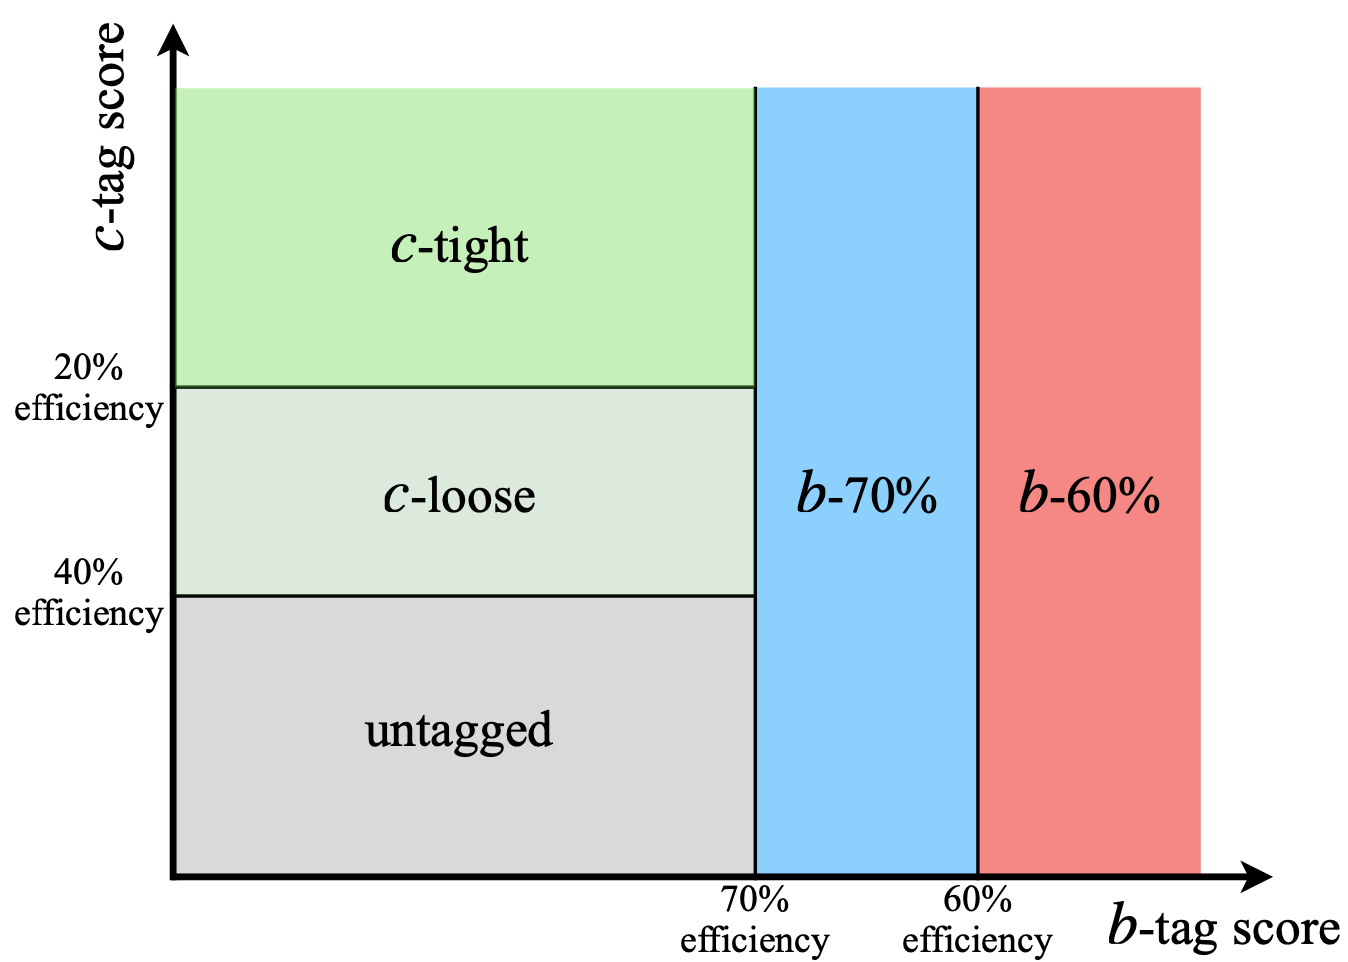
\includegraphics[width=0.98\textwidth]{Images/VH/pseudocontinuous.png}
      \end{minipage}
      \begin{minipage}[c]{0.3\textwidth}
        \caption{The \glsfirst{pcft} scheme used to simultaneously define 2 $b$-tagged, a tight $c$-tagged, a loose $c$-tagged, and a non-tagged bins, from the internal documentation. } 
        \label{fig:pseudotag}
      \end{minipage}
  \end{figure}
  \item The boosted regime only targets $b$-jets, following the single-purpose tagging used in the standard calibration of the tagger. As such, the standard pseudo-continuous $b$-tagging method is used. The track-jets associated to the leading large-$R$ jet are given a $b$-score based on the per-flavour probabilities outputted by \gls{dl1r}. The 85\% working point is adopted to maximise the signal yield, due to the important statistical limitations in the boosted regime. Track-jets passing this working point are $B$-tagged, otherwise they are untagged $N$. Studies showed that the very loose \gls{dl1r} \gls{wp} gives a better expected statistical significance than the then-available $X_{bb}$ tagger. The official calibration from Ref \cite{atlas:FTAGRUN2} is used, and extended to higher $p_T$ due to the wide range of $p_T$ probed in the analysis using uncertainty extrapolation, as presented in Appendix \ref{appsec-vh-ftagcal}.
\end{itemize}
While the analysis was underway, the superior single-jet \gls{gnn} taggers and the boosted objects $GN2X$ tagger introduced in Chapter \ref{chap-ftag} were not yet available as their calibration was an ongoing effort. Furthermore, switching to these new taggers was not feasible from a practical point of view in the timing of the analysis. They represent, however, an exciting avenue for progress in future iterations of this search, in both the resolved and boosted regimes. \\ % TODO check how the wp are defined %TODO also check the fc alue

\paragraph{Object Overlap:} overlap removal is applied to avoid double-counting electrons, muons, small-$R$ and large-$R$ jets, and hadronically decaying $\tau$'s that pass the object selection.

\subsection{Event Selection}\label{sec-regimeCat}
The trigger selections of the \vhb\ and \vhc\ have been harmonised for the combined analysis, and are specified per lepton channel in 0-lepton (0L), 1-lepton (1L), and 2-lepton (2L). Further details on the trigger setup are given in Table~\ref{aptab:trigs2015_to_2018} of the Appendix. In 0L, events are selected using the lowest un-prescaled \etm trigger, with increasing threshold rising from 70 GeV for data recorded in 2015, 90 to 110 GeV for 2016, and to 110 GeV for 2017 and 2018 due to higher trigger rate later in Run 3. The 1L channel triggers cover both the $e$ and the $\mu$ sub-channels. For the $e$-channel, single electron events must be triggered by the lwoest un-prescaled single electron triggers. For muons, the \etm trigger of 0L is used for events with \ptv\ > 150 GeV, while the lowest un-prescaled single muon trigger is used for events with a lower \ptv. Finally, the triggers for 2L are equivalent to 1L except for the muon channel where the \ptv\ threshold for switching between triggers is raised to 250 GeV. The use of \etm trigger at high \ptv\ for muons was shown to increase signal acceptancy by $\sim$ 5\%.\\ % TODO missing boosted no?


The different regimes of the analysis are defined by flavour tagging and the strategy to reconstruct the Higgs boson. In the resolved regime, an event must have at least two central jets. Two candidate jets are selected to reconstruct the Higgs using the so-called \textit{All Signal Jets} strategy, and define an event-tag by combining their individual tags. A hierarchy of tags is introduced, following the ordering: $B$ > $T$ > $L$ > $N$. The pair of candidates is selected from the two central jets having the highest tags, and the highest $p_T$ in case of ties. Events are labelled based on the tag of the selected jets, e.g., $TT$ is assigned to events with 2 tight $c$-tagged jet and $BL$ to events with a $b$-tagged and a loose $c$-tagged jets. In the boosted regime, at least to track-jets are required to be associated to the large-$R$ jet leading by $p_T$, and the tags of the 3 track-jets with the highest $p_T$ are considered for the event. This labelling and the reconstructed \ptv\ defines the different regimes of the resolved and boosted \vhb\ and \vhc\ parts of the cobpined analysis. To fully reconstruct the Higgs boson from the two candidates, additional selections are applied.

\paragraph{Higgs candidates in resolved regime:} for \vhb, the two candidates must be $b$-tagged (bins 3 and 4) with no additional $B$- and tight $c$-tagged jets allowed\footnote{In 2L, additional $T$-tagged jets are allowed due to the limited statistics and the different derivation of the top \gls{cr} in 2L, requiring mixed leptons $e\mu$.}, while in \vhc\ no $b$-tagged jets - neither candidate nor additional - is allowed and one of the candidate must have a tight $T$-tag. As described in the next section, two control regions are defined by changing this flavour selection: the topCR, combining a $B$-tag with a $T$-tag and the $V+l$ require loose $L$-tagged jet with an untagged $N$ jet for \vhc.. The Higgs candidates are sorted by $p_T$ into a leading $j_1$ and sub-leading $j_2$ candidates. The leading candidate must have $p_T > 45$ GeV, while other jets are required to have $p_T > 20 GeV$. The invariant mass of the Higgs candidate as measured by $m_{bb}$ ($m_{cc}$) for \vhb\ (\vhc) must be above 50 GeV before reconstruction techniques are applied to the candidate, to avoid the $V$+jets gluon splitting mis-modelling at low masses.  \\ %TODO bc overlap in 2L VHbb: tight c jets are allowed? % TODO check V+l has LL LN, ... % TODO the additional jet cut is not clearly mentioned in the text: it seems it's only 20 geV
\paragraph{Higgs candidates in boosted regime:} the selection requires exactly two $B$ tags among the at-most 3 leading track-jets by $p_T$ associated to the leading large-$R$. The reconstructed mass of the Higgs candidate based on the leading-$R$ jet mass is required to be $m_J > 50$ GeV with a leading large-$R$ jet $p_T > 250$ GeV. \\

In all regimes, the number of reconstructed charged lepton in the final state defines three channels as the 0-lepton (0L), 1-lepton (1L), and 2-lepton (2L). The objective of this leptonic selection is to reconstruct the associated $V$ boson. The selection of events in the resolved regime is presented in Table~\ref{tbl:VHbbccevSelTable} and in the boosted regime in Table~\ref{tbl:VHbbBoostevSelTable}. Additional channel-specific requirements are also introduced to limit backgrounds contamination and are reviewed in the rest of this section.

\subsubsection{Selection specific to the 0-lepton channel}\label{subsubsec-0Lsel}
In the 0-lepton chanenel, 0 $VH$-loose leptons should be selected and \etm should be larger than 150 GeV (250 GeV) in the resolved (boosted) regime to target a $Z \rightarrow \nu\nu$ (with $H \rightarrow b\bar{b}/c\bar{c}$). \\ % TODO Conflict in the main note: selection is 200 in text for boosted and 250 in the table.

In the resolved regime, the scalar sum of the jet $p_T$ in the events $S_T$ is required to be $> 120$ GeV ($> 150$ GeV) for 2-jets (3 or more jets) to avoid a mis-modelled region in simulation due to triggers. When a $W \rightarrow \tau \nu$ with a hadronic decay of the $\tau$-lepton reconstructed as a jet, no electron nor muon is reconstructed. To limit this fake $\tau$ contamination in the 0L channel, an extra selection is applied when at least 1 hadronic $\tau$ is reconstructed: the reconstructed transverse $W$ mass \[ m_T^W = \sqrt{2 p_T^l E_T^{\textrm{miss}} (1 - \cos(\Delta \phi(l, E_T^{\textrm{miss}} ) ) ) } \] is required to be higher than 10 GeV, with the $W$-boson $p_T$ estimated from the vectorial sum of the leading hadronic $\tau$ ($p_T^l$) and \etm instead of \ptv.

To limit the multi-jet background, so-called \textit{anti-QCD cuts} using the azimuthal angle $\phi$ are applied in all regimes:
\begin{itemize}
    \item For resolved only, $|\Delta \phi(j_1, j_2)| < 140 \ensuremath{^\circ}$.
    \item $|\Delta \phi(E_t^{\textrm{miss}}, H)| > 120 \ensuremath{^\circ}$,
    \item $\textrm{min}|\Delta \phi (E_T^{\textrm{miss}}, \textrm{ jet})|$ must be $> 20\ensuremath{^\circ}$ ($> 30 \ensuremath{^\circ}$) for resolved 2-jet (3-jet) events and $> 30\ensuremath{^\circ}$ for the boosted regime.
\end{itemize}
The cuts were tuned to limit the multi-jet contamination to a fraction of order 1\% of the total background in 0L. Consequently, the mutli-jet is deemed negligible in 0L. 

\subsubsection{Selection specific to the 1-lepton channel}
In the 1L channel, the targeted decaying vector boson is a $W \rightarrow \ell\nu$, with the $\ell = e, \mu$. Exactly 1 $WH$-signal lepton is required, with events having more than 1 $VH$-loose lepton vetoed. The vector boson is reconstructed from the vectorial sum of the \etm and the lepton tranverse momentum identified in the event, with a $p_T^W > 75$ GeV. To suppres the multi-jet background, events with an electron are required to have an \etm $>$ 30 GeV in the resolved and $> 50$ GeV in the boosted regime, with a reconstructed $m_T^W > 20$ GeV for events with low $W$ transverse momentum, $p_T^W \in [75, 150]$ GeV. For the resolved $\mu$-channel, as the same \etm trigger is used as in the 0L, the scalar sum of $p_T$ is similarly restrained as in 0L: $S_T > 120$ GeV ($> 150$ GeV) for 2-jets (3 or more jets). A significant background is the \ttb, with both $t$ decaying into a $W$ boson and a $b$-quark. Events where one of the $W$ boson decay follows $W \rightarrow \tau \nu$ with the $\tau$ decaying hadronically and the other $W$ decays into an $e$ or a $\mu$ have the same signature as the searched signal. A hadronic $\tau$-veto is applied in all regimes to suppress this background. Events passing the 0-lepton selection with $\geq 1$ hadronic taus are moved to the 1-lepton channel with the leading hadronic $tau$ used to reconstruct variables requiring an $e/\mu$. This migration is performed to recover the estimated $~10$\% ($\sim$ 20\%) of $WH$ signal with $W\rightarrow \tau \nu$ with hadronically decaying $\tau$-lepton in the resolved (boosted) regime and decorrelated the 0L and 1L channels.

\subsubsection{Selection specific to the 2-lepton channel}
The 2L channel targets the associated bosonic decay $Z \rightarrow\ell\ell$, with the $Z$ reconstructed from two $VH$-loose leptons required to have the same flavour, with at least one passing the $VH$-signal lepton requirements. In the di-muon channel, the leptons are further required to be of opposite charge\footnote{This is not applied to the di-electron system due to the higher charge mis-identification.}. The invariant mass of the di-lepton system is required to be consistent with the $Z$ mass with $81 < m_{ll} < 101$ GeV in resolved and $66 < m_{ll} < 111$ GeV in boosted, to suppress non-resonant lepton-pair producing background, such a \ttb\ and multi-jet. The leptons must satisfy $p_T > 25$ GeV and the stricter $p_T > 27$ GeV for the leading muon when the event is selected by the muon trigger.

\clearpage
%
% From: https://gitlab.cern.ch/atlas-physics-office/HIGG/ANA-HIGG-2020-20/ANA-HIGG-2020-20-INT1/-/blob/master/Tex/Texsection/Selection/VHbbccevSelTable.tex
\begin{table}[h!]
    \begin{center}
    \begin{tabular}{C{6cm}|C{4cm}|C{4cm}}
    \hline \hline
    Resolved Analysis Regime & $VH(H\rightarrow b\bar{b})$ & $VH(H\rightarrow c\bar{c})$ \\
    \hline \hline
    \multicolumn{1}{c}{}  &\multicolumn{2}{c}{Common Selections}\\ \hline 
    Jets & \multicolumn{2}{c}{$\geq$ 2 signal jets}  \\
    Candidate jets tagging &  2 $B$-tags & $\geq1$ $T$-tag, no $B$-tag \\
    Leading Higgs ($H$) candidate jet $p_T$ & \multicolumn{2}{c}{$>$ 45 GeV} \\
    Sub-leading $H$ candidate jet $p_T$ & \multicolumn{2}{c}{$>$ 20 GeV} \\
    $m_{bb}$ or $m_{cc}$ & \multicolumn{2}{c}{> 50 GeV (before correction)} \\ 
    Non-$H$ candidate jet $p_T$ & \multicolumn{2}{c}{$>$ 20 GeV ($> 30$ GeV for nJet categorisation only)} \\ % TODO seems to be gone and fixed at 20 
    Candidate jets $\Delta R$  & \multicolumn{2}{c}{Upper cut $\Delta R \leq \pi$} \\

    \hline \hline 
    \multicolumn{1}{c}{} &\multicolumn{2}{c}{0-Lepton} \\
    \hline
    Trigger & \multicolumn{2}{c}{$E_T^{\textrm{miss}}$ triggers} \\
    Jets & $\leq$ 4 jets & $\leq$ 3 jets \\
    Additional jets tagging & no $T$-tag & no $B$-tag \\
    Top CR tagging & \multicolumn{2}{c}{$\geq$1 $B$-tag + 1 $T$-tag} \\
    Leptons & \multicolumn{2}{c}{0 $VH$-loose lepton} \\
    $E_T^{\textrm{miss}}$ & \multicolumn{2}{c}{$>$ 150~GeV}  \\
    $E_{T, trk}^{\textrm{miss}}$  & - & $>$ 30~GeV \\
    $S_T = \sum p_T^{\textrm{jets}}$ & \multicolumn{2}{c}{$>$ 120 GeV (2 jets), $>$150 GeV ($\geq3$ jets)}  \\ % Adapt: in object introduce S_T
    $m_T^W$ & \multicolumn{2}{c}{$>$ 10 GeV when $\geq$ 1 hadronic $\tau$} \\
    $|\Delta\phi(j_1, j_2)|$ & \multicolumn{2}{c}{$< 140\ensuremath{^\circ}$} \\
    $|\Delta\phi(E_T^{\textrm{miss}}, H)|$ & \multicolumn{2}{c}{$> 120\ensuremath{^\circ}$} \\
    $\textrm{min}|\Delta \phi (E_T^{\textrm{miss}}, \textrm{jet})|$& \multicolumn{2}{c}{$>20\ensuremath{^\circ}$ (2 jets), $> 30\ensuremath{^\circ}$(3 jets)} \\
    %$|\Delta\phi(E_T^{\textrm{miss}},E_{T, trk}^{\textrm{miss}})|$ & \multicolumn{2}{c}{$< 90\ensuremath{^\circ}$} \\ % TODO this is missing from the table and not mentioned in the text

    \hline\hline 
    \multicolumn{1}{c}{} & \multicolumn{2}{c}{1-Lepton} \\
    \hline
    Trigger &  \multicolumn{2}{c}{$e$-channel: single electron trigger} \\
            & \multicolumn{2}{c}{$\mu$-channel: single muon trigger ($p_T^V <$ 150 GeV)} \\
            & \multicolumn{2}{c}{and 0L $E_T^{\textrm{miss}}$ triggers} \\
    Jets & \multicolumn{2}{c}{$\leq$ 3 jets}  \\
    Additional jets tagging & no $T$-tag & no $B$-tag \\
    Top CR tagging & \multicolumn{2}{c}{$\geq$1 $B$-tag + 1 $T$-tag} \\ % TODO fix the footnoteref
    hadronic $\tau$-veto & \multicolumn{2}{c}{no hadronic $\tau$} \\ 
    Leptons & \multicolumn{2}{c}{1 $WH$-signal lepton} \\
            &  \multicolumn{2}{c}{$>1$~$VH$-loose lepton veto} \\
    $E_T^{\textrm{miss}}$   & \multicolumn{2}{c}{$>$ 30~GeV ($e$ channel)} \\
    $S_T$ & \multicolumn{2}{c}{Same as 0L for $\mu$ with \etm trigger}  \\ 
    $m_T^W$ & \multicolumn{2}{c}{$>$ 20 GeV for 75 < \ptv\ < 150 GeV} \\ % TODO, in text it says 20 GeV, but table says 10

    \hline\hline 
    \multicolumn{1}{c}{} & \multicolumn{2}{c}{2-Lepton}\\
    \hline
    Trigger &  \multicolumn{2}{c}{Same as 1L, \ptv\ $<$ 250 GeV for single $\mu$ trigger}\\
    Additional jets tagging & - & no $B$-tag \\
    Leptons & \multicolumn{2}{c}{2 $VH$-loose leptons} \\
            & \multicolumn{2}{c}{($\geq$ 1 $ZH$-signal lepton)} \\
            & \multicolumn{2}{c}{Same flavour, opposite-charge for $\mu\mu$} \\
    Top CR  & \multicolumn{2}{c}{Mixed $e\mu$ flavour} \\ 
    $m_{ll}$   & \multicolumn{2}{c}{81 $<$ $m_{ll}$ $<$ 101~GeV} \\
    %$E_T^{\textrm{miss}}$ significance (cut-based)  & \multicolumn{2}{c}{E_T^{\textrm{miss}}$/\sqrt{\textrm{HT}} < 3.5\sqrt{GeV}$} \\
    \hline\hline

    \end{tabular}
    \caption{Summary of the event selection in the 0-, 1- and 2-lepton channels of the resolved \vhbc regimes, adapted from the internal documentation. The common Top CR tagging definition ignore the candidate jet tagging requirements. For \vhc, an extra CR for $V+l$ changes the candidate tagging to one $L$-tag + no $T$-tag ($LN$).} % TODO ADAPT THE LEGEND FOR WHAT IS PRESENTED
    % There was also: Variables not presented in the text: $E_{T, trk}^{\textrm{miss}}$ is the missing transverse momentum calculated from the negative vector sum of the transverse momenta of tracks reconstructed in the inner detector and identified as originating from the primary vertex
    \label{tbl:VHbbccevSelTable}
    \end{center}
\end{table}
%

\begin{table}[htbp]
    \hspace{-0.6cm}
    \begin{tabular}{C{3cm}|C{2.95cm}|C{2.5cm}|C{1.8cm}|C{2.5cm}|C{1.8cm}}
    \hline \hline
    Selection & 0-Lepton & \multicolumn{2}{c|}{1-Lepton} & \multicolumn{2}{c}{2-Lepton}  \\
    & & $e$-channel & $\mu$-channel & $e$-channel & $\mu$-channel \\ \hline \hline
    Trigger & \etm & Single electron & \etm & Single electron & \etm \\
    Leptons & 0 $VH$-loose lepton & \multicolumn{2}{c|}{1 $WH$-signal lepton} & \multicolumn{2}{c}{$\geq$ 1 $ZH$-signal lepton} \\
     & & \multicolumn{2}{c|}{No second $VH$-loose lepton} & \multicolumn{2}{c}{2 $VH$-loose leptons} \\
     &  & \multicolumn{2}{c|}{No hadronic $\tau$} & \multicolumn{2}{c}{Same flavour leptons} \\
     &  &  \multicolumn{2}{c|}{} & \multicolumn{2}{c}{Opposite charge for $\mu\mu$} \\ \hline
    \ptv\ &  \multicolumn{5}{c}{$>$ 400 GeV} \\
    Large-$R$ jet & \multicolumn{5}{c}{$\geq$ 1 large-$R$ jet ($R$ = 1.0), $p_T >$ 250 GeV, $|\eta| < 2$} \\
    Track-Jets & \multicolumn{5}{c}{$\geq$ 2 track-jets ($p_T > 10$ GeV, $|\eta| < 2.5$) matched to the leading large-$R$ jet} \\
    Tagging & \multicolumn{5}{c}{Exactly 2 of the 3 leading track-jets matched to the large-$R$ jet must be $b$-tagged} \\
    $m_J$ & \multicolumn{5}{c}{$> 50$ GeV} \\ \hline
    \etm & $>$ 200 GeV & $>$ 50 GeV & - & \multicolumn{2}{c}{-} \\ % TODO For 0L, it's 200 in the text but 250 in the table
    $|\Delta\phi(E_T^{\textrm{miss}}, H)|$ & $> 120\ensuremath{^\circ}$ & \multicolumn{2}{c|}{-} & \multicolumn{2}{c}{-} \\
    $\min |\Delta\phi(E_T^{\textrm{miss}}, \textrm{jets})|$ & $> 30\ensuremath{^\circ}$ & \multicolumn{2}{c|}{-} & \multicolumn{2}{c}{-} \\
    $m_{ll}$ & - & \multicolumn{2}{c|}{-} &  \multicolumn{2}{c}{$66$ GeV $< m_{ll} < 116 $ GeV} \\ \hline \hline
    \end{tabular}
    \caption{Summary of the event selection in the 0-, 1- and 2-lepton channels of the boosted \vhb\ regime, adapted from the internal documentation.} % TODO ADAPT THE LEGEND FOR WHAT IS PRESENTED
    \label{tbl:VHbbBoostevSelTable}
\end{table}


\subsection{Event Categorisation}\label{sec-eventCat}
% TODO topCR here, say the candidates are highest pT B and highest pT T
Events are futher categorised following a successive decomposition into regions of defined tag, vector boson $V$ transverse momentum $p_T^V$, and number of jets (both central and forward). The full categorisation gives rise to signal and control regions that enter the statistical analysis defined in the fit framework of Section \ref{sec-fitFramework}. The control regions are defined to help constrain the modelling of specific backgrounds and the correct their yields. The definition of the regions depend on the analysis regime and the targeted Higgs decay, with Figure \ref{fig:ana-strat-det} providing a global overview of the different regions defined.

\subsubsection{Resolved Regime Categorisation}
In the resolved regime, the number of central + forward jets in an event defines different categories to maximise the signal sensitivity. A $p_T > 30$ GeV cut is considered for non-Higgs candidate jets just to determine the number of jet categorisation. This was found to limit the signal migration across \gls{stxs} bins in \vhb\ while having almost no impact on the \vhc\ sensitivity\footnote{It is nonetheless applied to harmonise the resolved regime.}.All distributions of the resolved regime regions entering the fit are presented in Appendix \ref{appsec-vh-analRegRes}.

\paragraph{Resolved \vhb:} requires exactly 2 $b$-tagged jets ($BB$), with no extra $B$ nor any $T$, and events are separated into different categories based on central + forward jet multiplicity. All lepton channels have a 2-jet and 3-jet categories. The 0L channel has an addittional 4-jet category and the 2L an extra 4 or more jets (4p) category\footnote{The 4/4p-jet category in 1L overlaps with the region used to calibrate the tagger and is rejected due to the \ttb\ limiting the sensitivity.}. They are included for more sensitive \gls{stxs} measurements in bins with more than one additional jets. The regions are also split in different bins of $p_T^V$ as [75, 150] GeV (except for 0L\footnote{It is not feasible in 0L due to the trigger threshold on $E_T^{\textrm{miss}}$.}), [150, 250] GeV, and [250, 400] GeV. Some \vhb\ signal regions to the analysis are presented here in Figure \ref{fig:plots_VHbb_ex_SR}. The distributions presented in this section corresponds to the variables chosen for the fit, and are described further in Section \ref{sec-vh-disc}.

\begin{figure}[h!]
  \centering
  \begin{subfigure}[b]{0.32\textwidth}
      \centering
      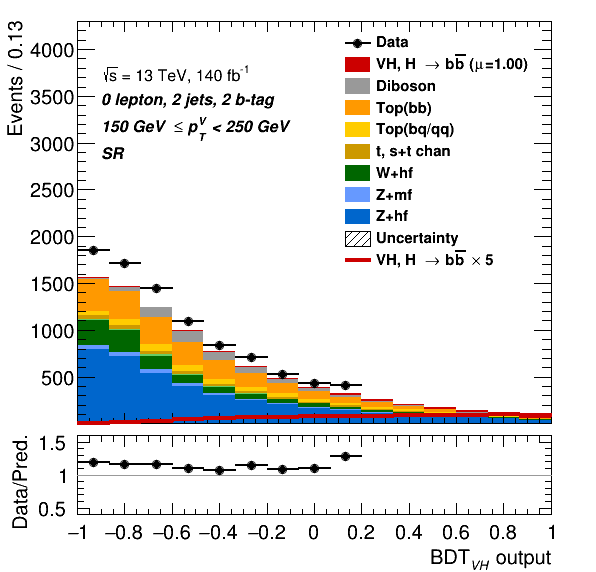
\includegraphics[width=\textwidth]{Images/VH/Own_fit/prefit_VHbb/Region_distmva_BMax250_BMin150_DSR_J2_TTypebb_T2_L0_Y6051_Prefit.png}
      \caption{0-lepton.}
      \label{fig:plots_VHbb_ex_OL_SR}
  \end{subfigure}
  \begin{subfigure}[b]{0.32\textwidth}
      \centering
      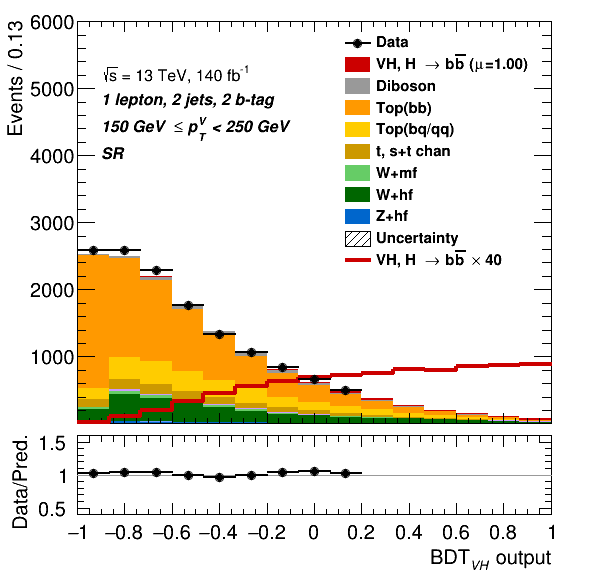
\includegraphics[width=\textwidth]{Images/VH/Own_fit/prefit_VHbb/Region_distmva_BMax250_BMin150_DSR_J2_TTypebb_T2_L1_Y6051_Prefit.png}
      \caption{1-lepton}
      \label{fig:plots_VHbb_ex_1L_SR}
  \end{subfigure}
  \begin{subfigure}[b]{0.32\textwidth}
    \centering
    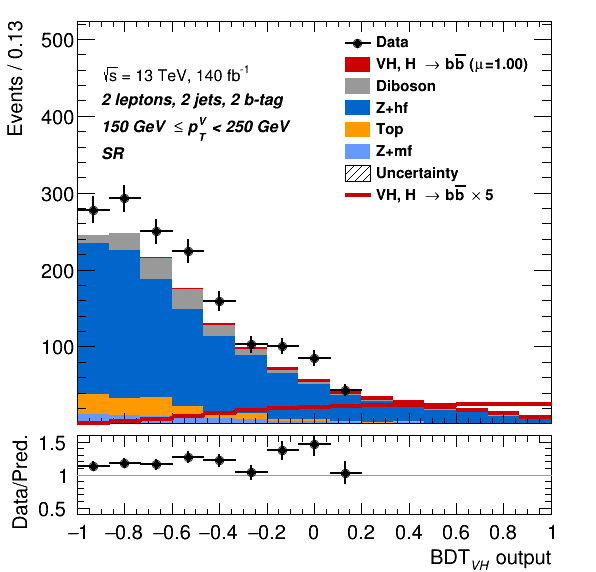
\includegraphics[width=\textwidth]{Images/VH/Own_fit/prefit_VHbb/Region_distmva_BMax250_BMin150_DSR_J2_TTypebb_T2_L2_Y6051_Prefit.png}
    \caption{2-lepton.}
    \label{fig:plots_VHbb_ex_2L_SR}
\end{subfigure}
  \caption{The $BB$-tagged 2-jet 150 < \ptv\ < 250 GeV signal regions in the different lepton channels.}
  \label{fig:plots_VHbb_ex_SR}
\end{figure} 


\paragraph{Resolved \vhc:} adopts a similar event categorisation to the resolved \vhb, with now at least one candidate jet being tight c-tagged. The categorisation of the signal region is split based on the remaining candidate tag into a 2 $c$-tags region and a 1 $c$-tag region: the former requiring an extra loose ($LT$) or tight $c$-tag ($TT$), the latter an additional non-tagged jet $N$ ($NT$). The $p_T^V$ bins are similar to \vhb, except for the higgest $p_T^V$ one that is relaxed to $\geq 250$ GeV given the limited impact of the overlap with the boosted \vhb. Adding the \ptv\ region above 400 GeV was found to increase the total \vhc\ sensitivity by 10\%. The jet multiplicity is used to define a 2 and a 3 jets categories, with the latter being 3 or more jets (3p) in 2L only thanks to a reduced \ttb\ background. A selection of 2 $c$-tags signal regions is presented in Figure \ref{fig:plots_VHcc_ex_SR_2C}, with Figure \ref{} presenting some 1 $c$-tag signal regions.

\begin{figure}[h!]
  \centering
  \begin{subfigure}[b]{0.32\textwidth}
      \centering
      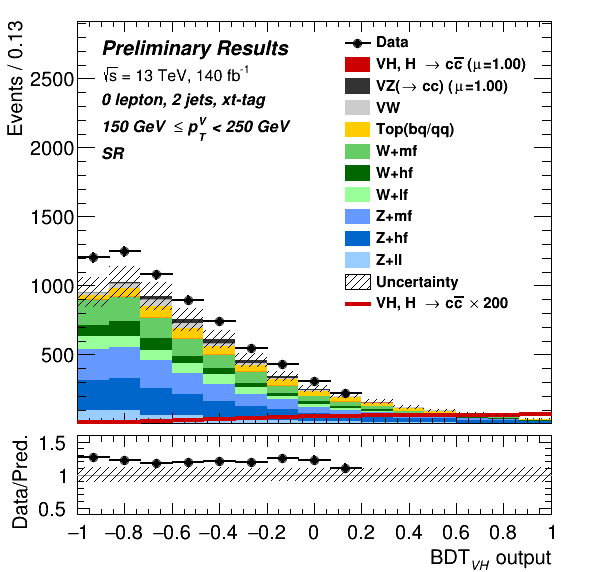
\includegraphics[width=\textwidth]{Images/VH/Own_fit/prefit_VHcc/Region_distmva_BMax250_BMin150_DSR_J2_TTypext_T2_L0_Y6051_Prefit.png}
      \caption{0-lepton, 2-jet.}
      \label{fig:plots_VHcc_ex_OL_SR_2C}
  \end{subfigure}
  \begin{subfigure}[b]{0.32\textwidth}
      \centering
      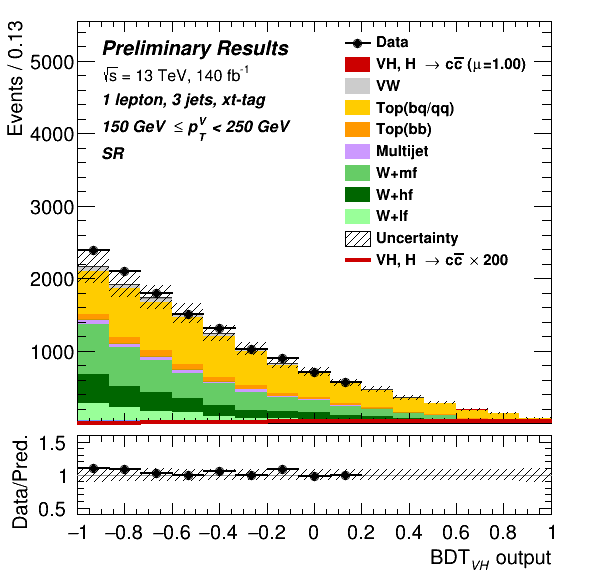
\includegraphics[width=\textwidth]{Images/VH/Own_fit/prefit_VHcc/Region_distmva_BMax250_BMin150_DSR_J3_TTypext_T2_L1_Y6051_Prefit.png}
      \caption{1-lepton, 3-jet.}
      \label{fig:plots_VHcc_ex_1L_SR_2C}
  \end{subfigure}
  \begin{subfigure}[b]{0.32\textwidth}
    \centering
    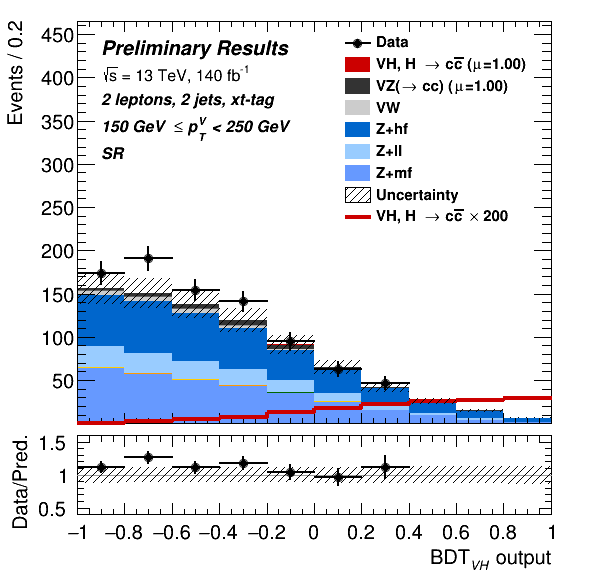
\includegraphics[width=\textwidth]{Images/VH/Own_fit/prefit_VHcc/Region_distmva_BMax250_BMin150_DSR_J2_TTypext_T2_L2_Y6051_Prefit.png}
    \caption{2-lepton, 2-jet.}
    \label{fig:plots_VHcc_ex_2L_SR_2C}
\end{subfigure}
  \caption{Some 2 $c$-tagged ($TT$ or $LT$) 150 < \ptv\ < 250 GeV signal regions in the different lepton channels.}
  \label{fig:plots_VHcc_ex_SR_2C}
\end{figure} 


\begin{figure}[h!]
  \centering
  \begin{subfigure}[b]{0.32\textwidth}
      \centering
      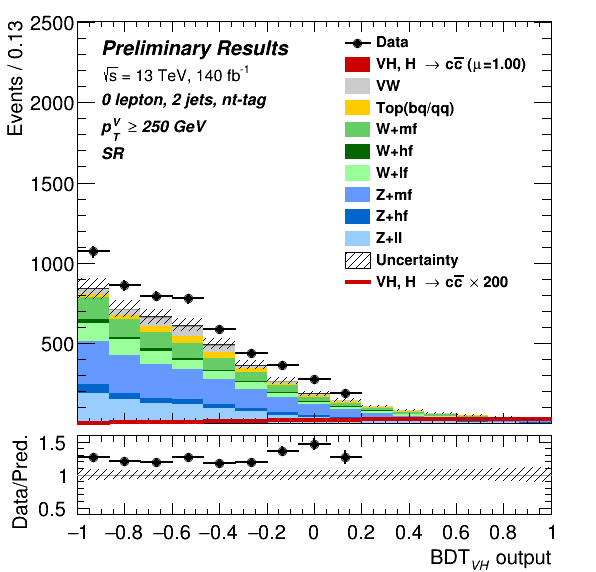
\includegraphics[width=\textwidth]{Images/VH/Own_fit/prefit_VHcc/Region_distmva_BMin250_DSR_J2_TTypent_T1_L0_Y6051_Prefit.png}
      \caption{0-lepton, 2-jet.}
      \label{fig:plots_VHcc_ex_OL_SR_1C}
  \end{subfigure}
  \begin{subfigure}[b]{0.32\textwidth}
      \centering
      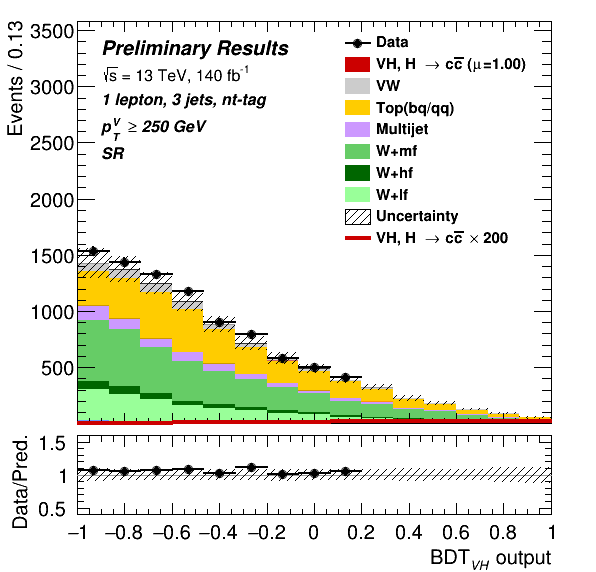
\includegraphics[width=\textwidth]{Images/VH/Own_fit/prefit_VHcc/Region_distmva_BMin250_DSR_J3_TTypent_T1_L1_Y6051_Prefit.png}
      \caption{1-lepton, 3-jet.}
      \label{fig:plots_VHcc_ex_1L_SR_1C}
  \end{subfigure}
  \begin{subfigure}[b]{0.32\textwidth}
    \centering
    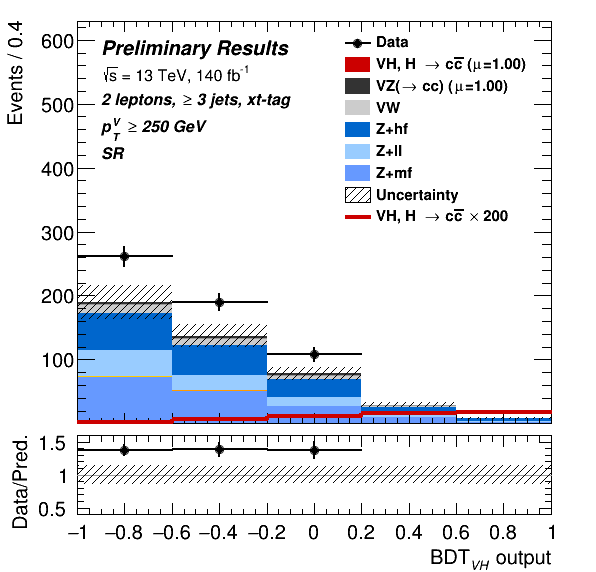
\includegraphics[width=\textwidth]{Images/VH/Own_fit/prefit_VHcc/Region_distmva_BMin250_DSR_J3_TTypext_incJet1_T2_L2_Y6051_Prefit.png}
    \caption{2-lepton, $\geq$ 3 jets.}
    \label{fig:plots_VHcc_ex_2L_SR_1C}
\end{subfigure}
  \caption{Some 1 $c$-tagged 250 < \ptv signal regions in the different lepton channels.}
  \label{fig:plots_VHcc_ex_SR_1C}
\end{figure} 



\paragraph{The High $\Delta R$ Control region:} is designed to constrain the $V+$jets and \ttb\ background in \vhb\ normalisation and shape. It is defined by a further categorisation based on the angular separation $\Delta R(j_1, j_2)$\footnote{$\Delta R(j_1, j_2) = \sqrt{(\eta_{j_1} - \eta_{j_2})^2 + (\phi_{j_1} - \phi_{j_2})^2 }$.} between the Higgs-candidate jets. This split is governed by a $p_T^V$ dependent cut on the $\Delta R$ that is derived to give a specific signal purity in the \gls{sr}: 95\% (85\%) of the signal should enter the \gls{sr} in the 2-jet (3 or more jets) category. The mathematical expression of the cuts are presented in Table \ref{tbl:CRhigh_definition}, and illustrated in Figure~\ref{fig:drccptvCutsVHcc} with more details in Appendix~\ref{ap-sec-vh-deltaR}. Events with a $\Delta R$ below the cutting line enter the signal region, while those above go in the \highdr\ \gls{cr}, also called \textit{HighCR}. To avoid some mis-modeling effect at \highdr\ and keep the \highdr\ \gls{cr} kinematically close to the \gls{sr}, an upper cut of $\Delta R = \pi$ is applied to all events. This effectively remove $\sim 40$\% of events in the \highdr\ \gls{cr} with negligible impact on the signal region. For \vhc, the $TT$ and $LT$ events are separated in the HighCR to constrain the $V+$hf and $V$+mf, while they are merged into the 2 $c$-tags in the \gls{sr}. In \vhb, the HighCRs are used to extract the normalisation of the backgrounds while in \vhc\ the shape of the $m_{c\bar{c}}$ or \ptv\ spectrum are also used. Some \highdr\ \gls{cr}s are shown in Figure \ref{fig:plots_VHcc_ex_CRH}.

\begin{table}[htbp]
    \centering
    \begin{tabular}{c|c|c}
      \hline
      \hline
      Category & \highdr\ Cut & \lowdr Cut\\ \hline
      $2-jet$ & $ \Delta R > 0.787 + e^{1.387 - 0.0070 \times p_{T}^{V} } $      &  $ \Delta R < 0.410 + e^{ 0.818 - 0.0106  \times p_{T}^{V} } $        \\
      $3-jet$ & $ \Delta R > 0.684 + e^{1.204 - 0.0060 \times p_{T}^{V} } $      &  $ \Delta R < 0.430 + e^{ 0.399 - 0.0093  \times p_{T}^{V} } $        \\
      $4-jet$ & $ \Delta R > 0.863 + e^{0.984 - 0.0041 \times p_{T}^{V} } $ &  $ \Delta R < 0.411 + e^{ 1.204 - 0.0060  \times p_{T}^{V} } $        \\
      $5p-jet$ & $ \Delta R > 1.667 + e^{0.519 - 0.0050 \times p_{T}^{V} } $ &  $ \Delta R < 0.501 + e^{ 1.192 - 0.0075  \times p_{T}^{V} } $      \\
      \hline
      \hline
    \end{tabular}
    \caption{Cuts defining the \highdr\ (centre) and \lowdr (right) control regions (CRHigh and CRLow).}
    \label{tbl:CRhigh_definition}
  \end{table}
  
\begin{figure}[h!]
    %\hspace{-2.0cm}
    \center
    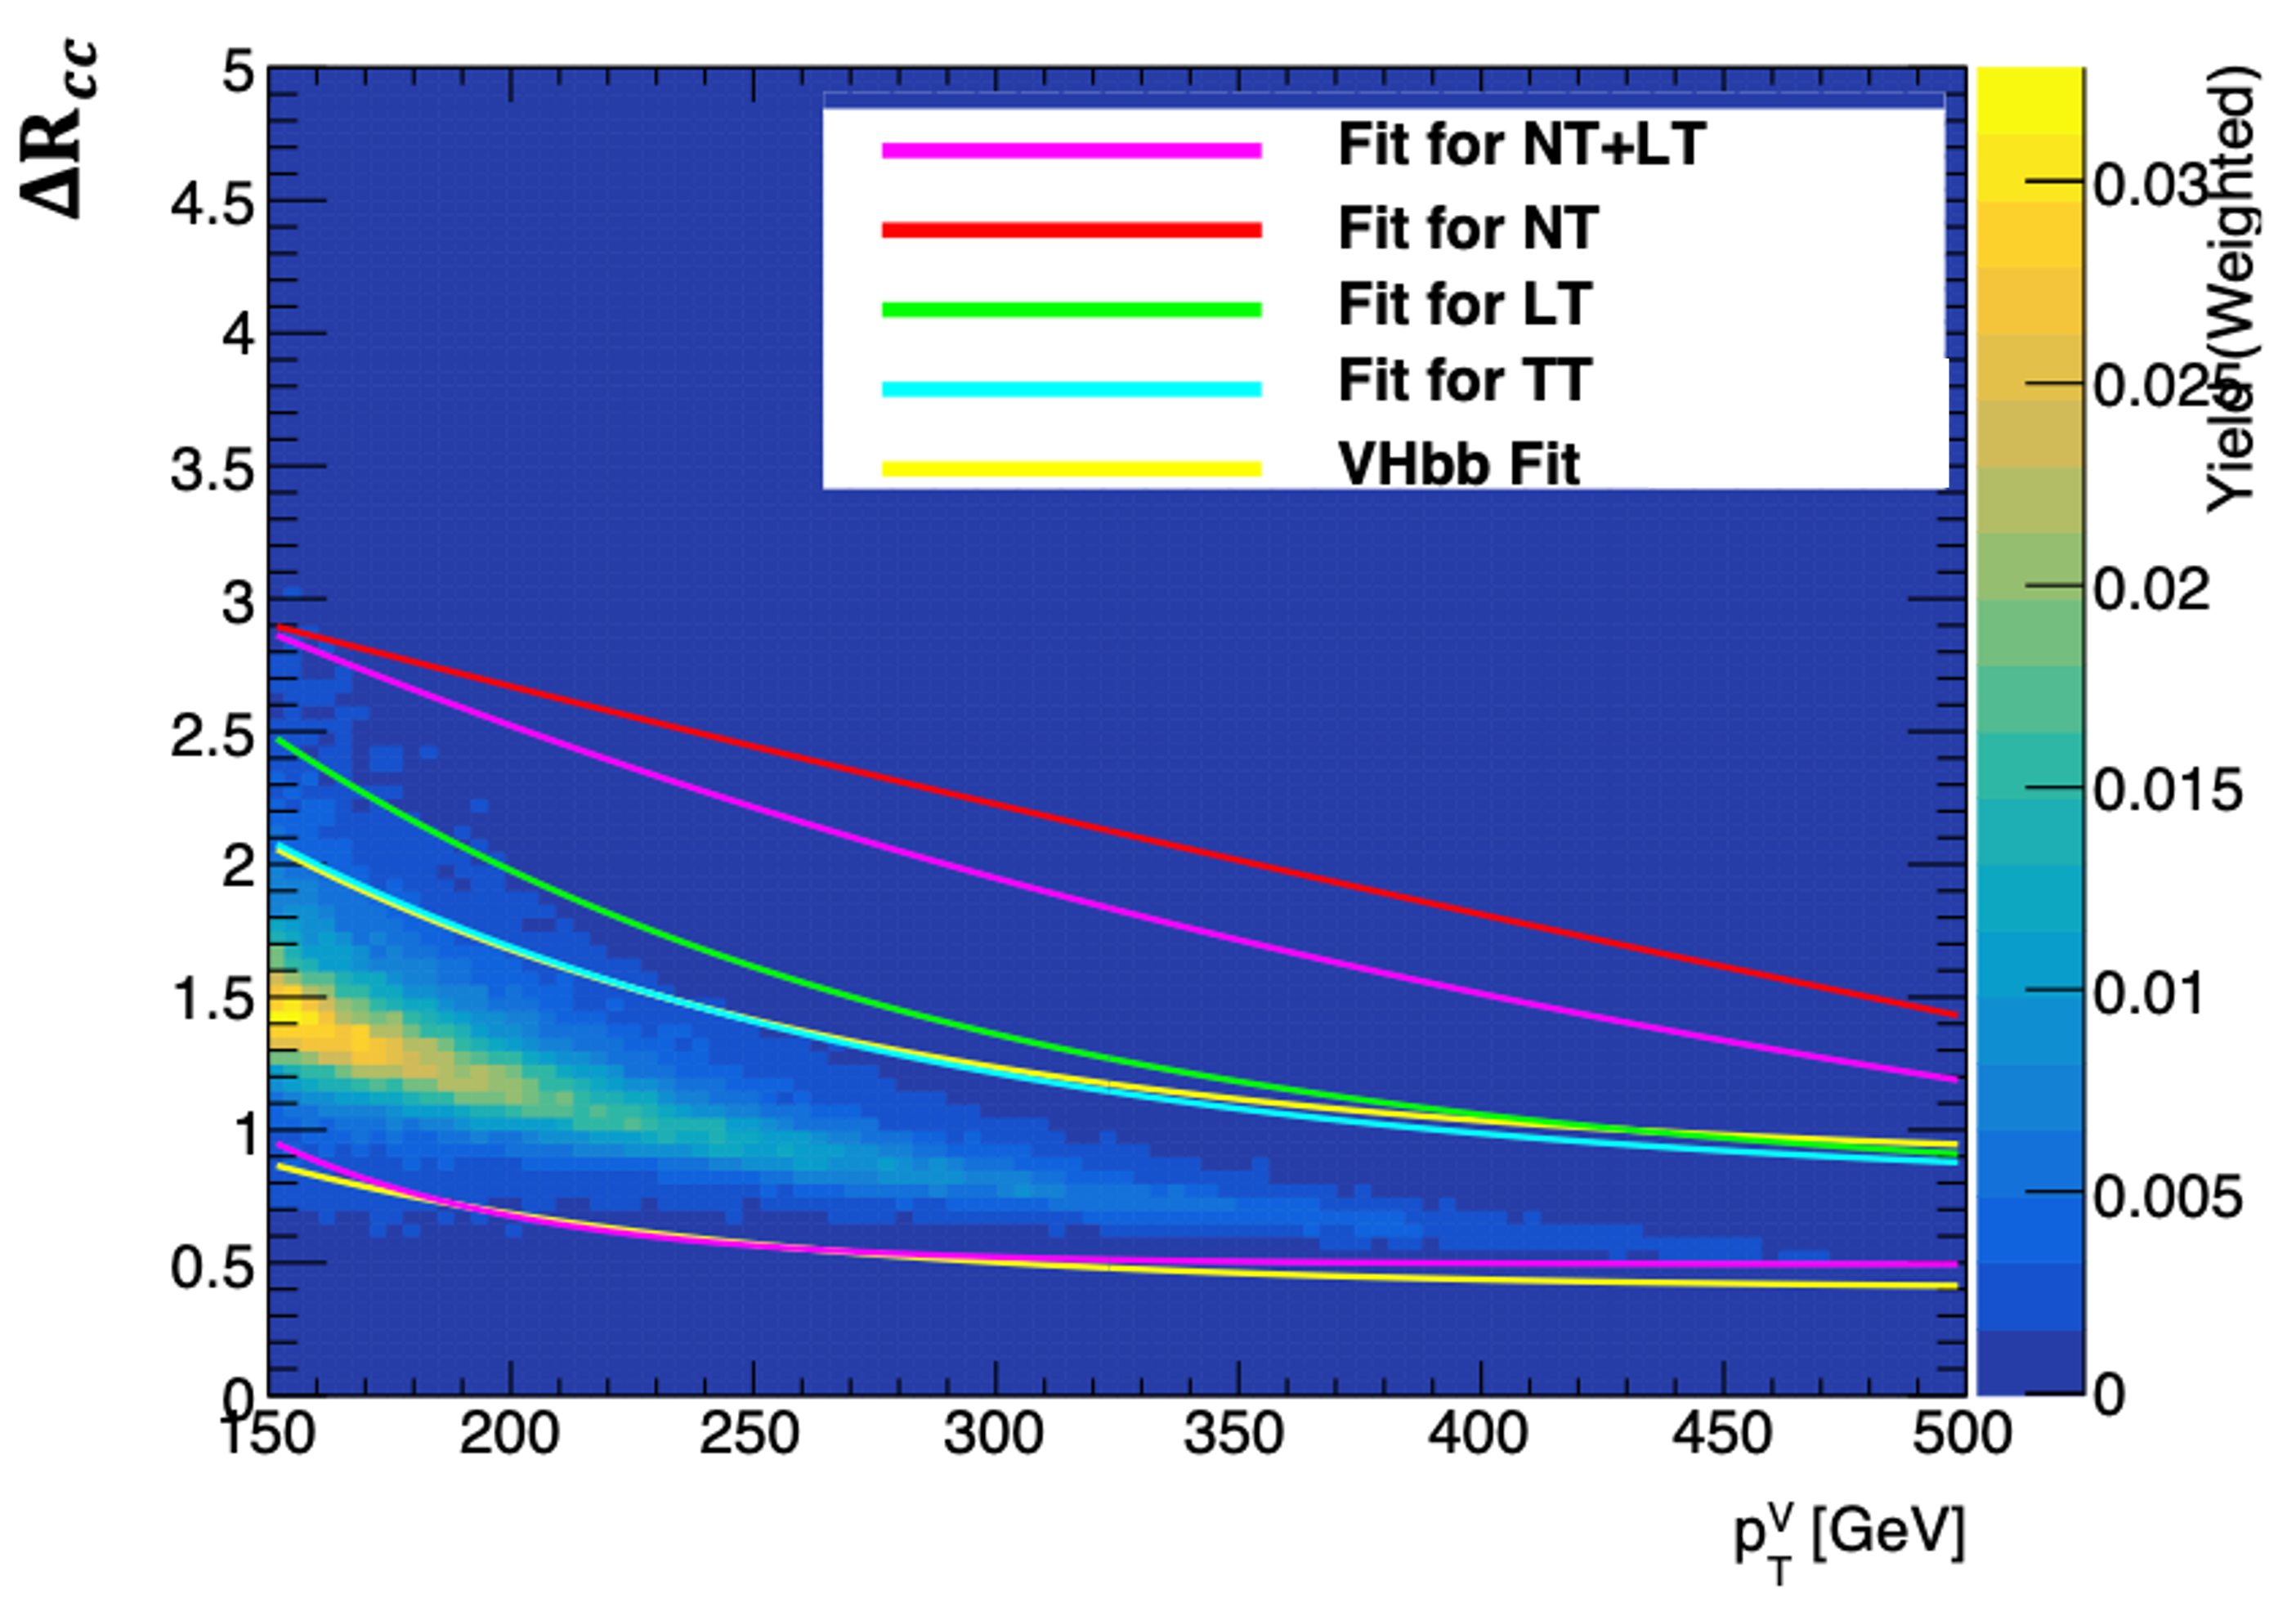
\includegraphics[width=0.48\textwidth]{Images/VH/dRccpTV/sr1.png}
    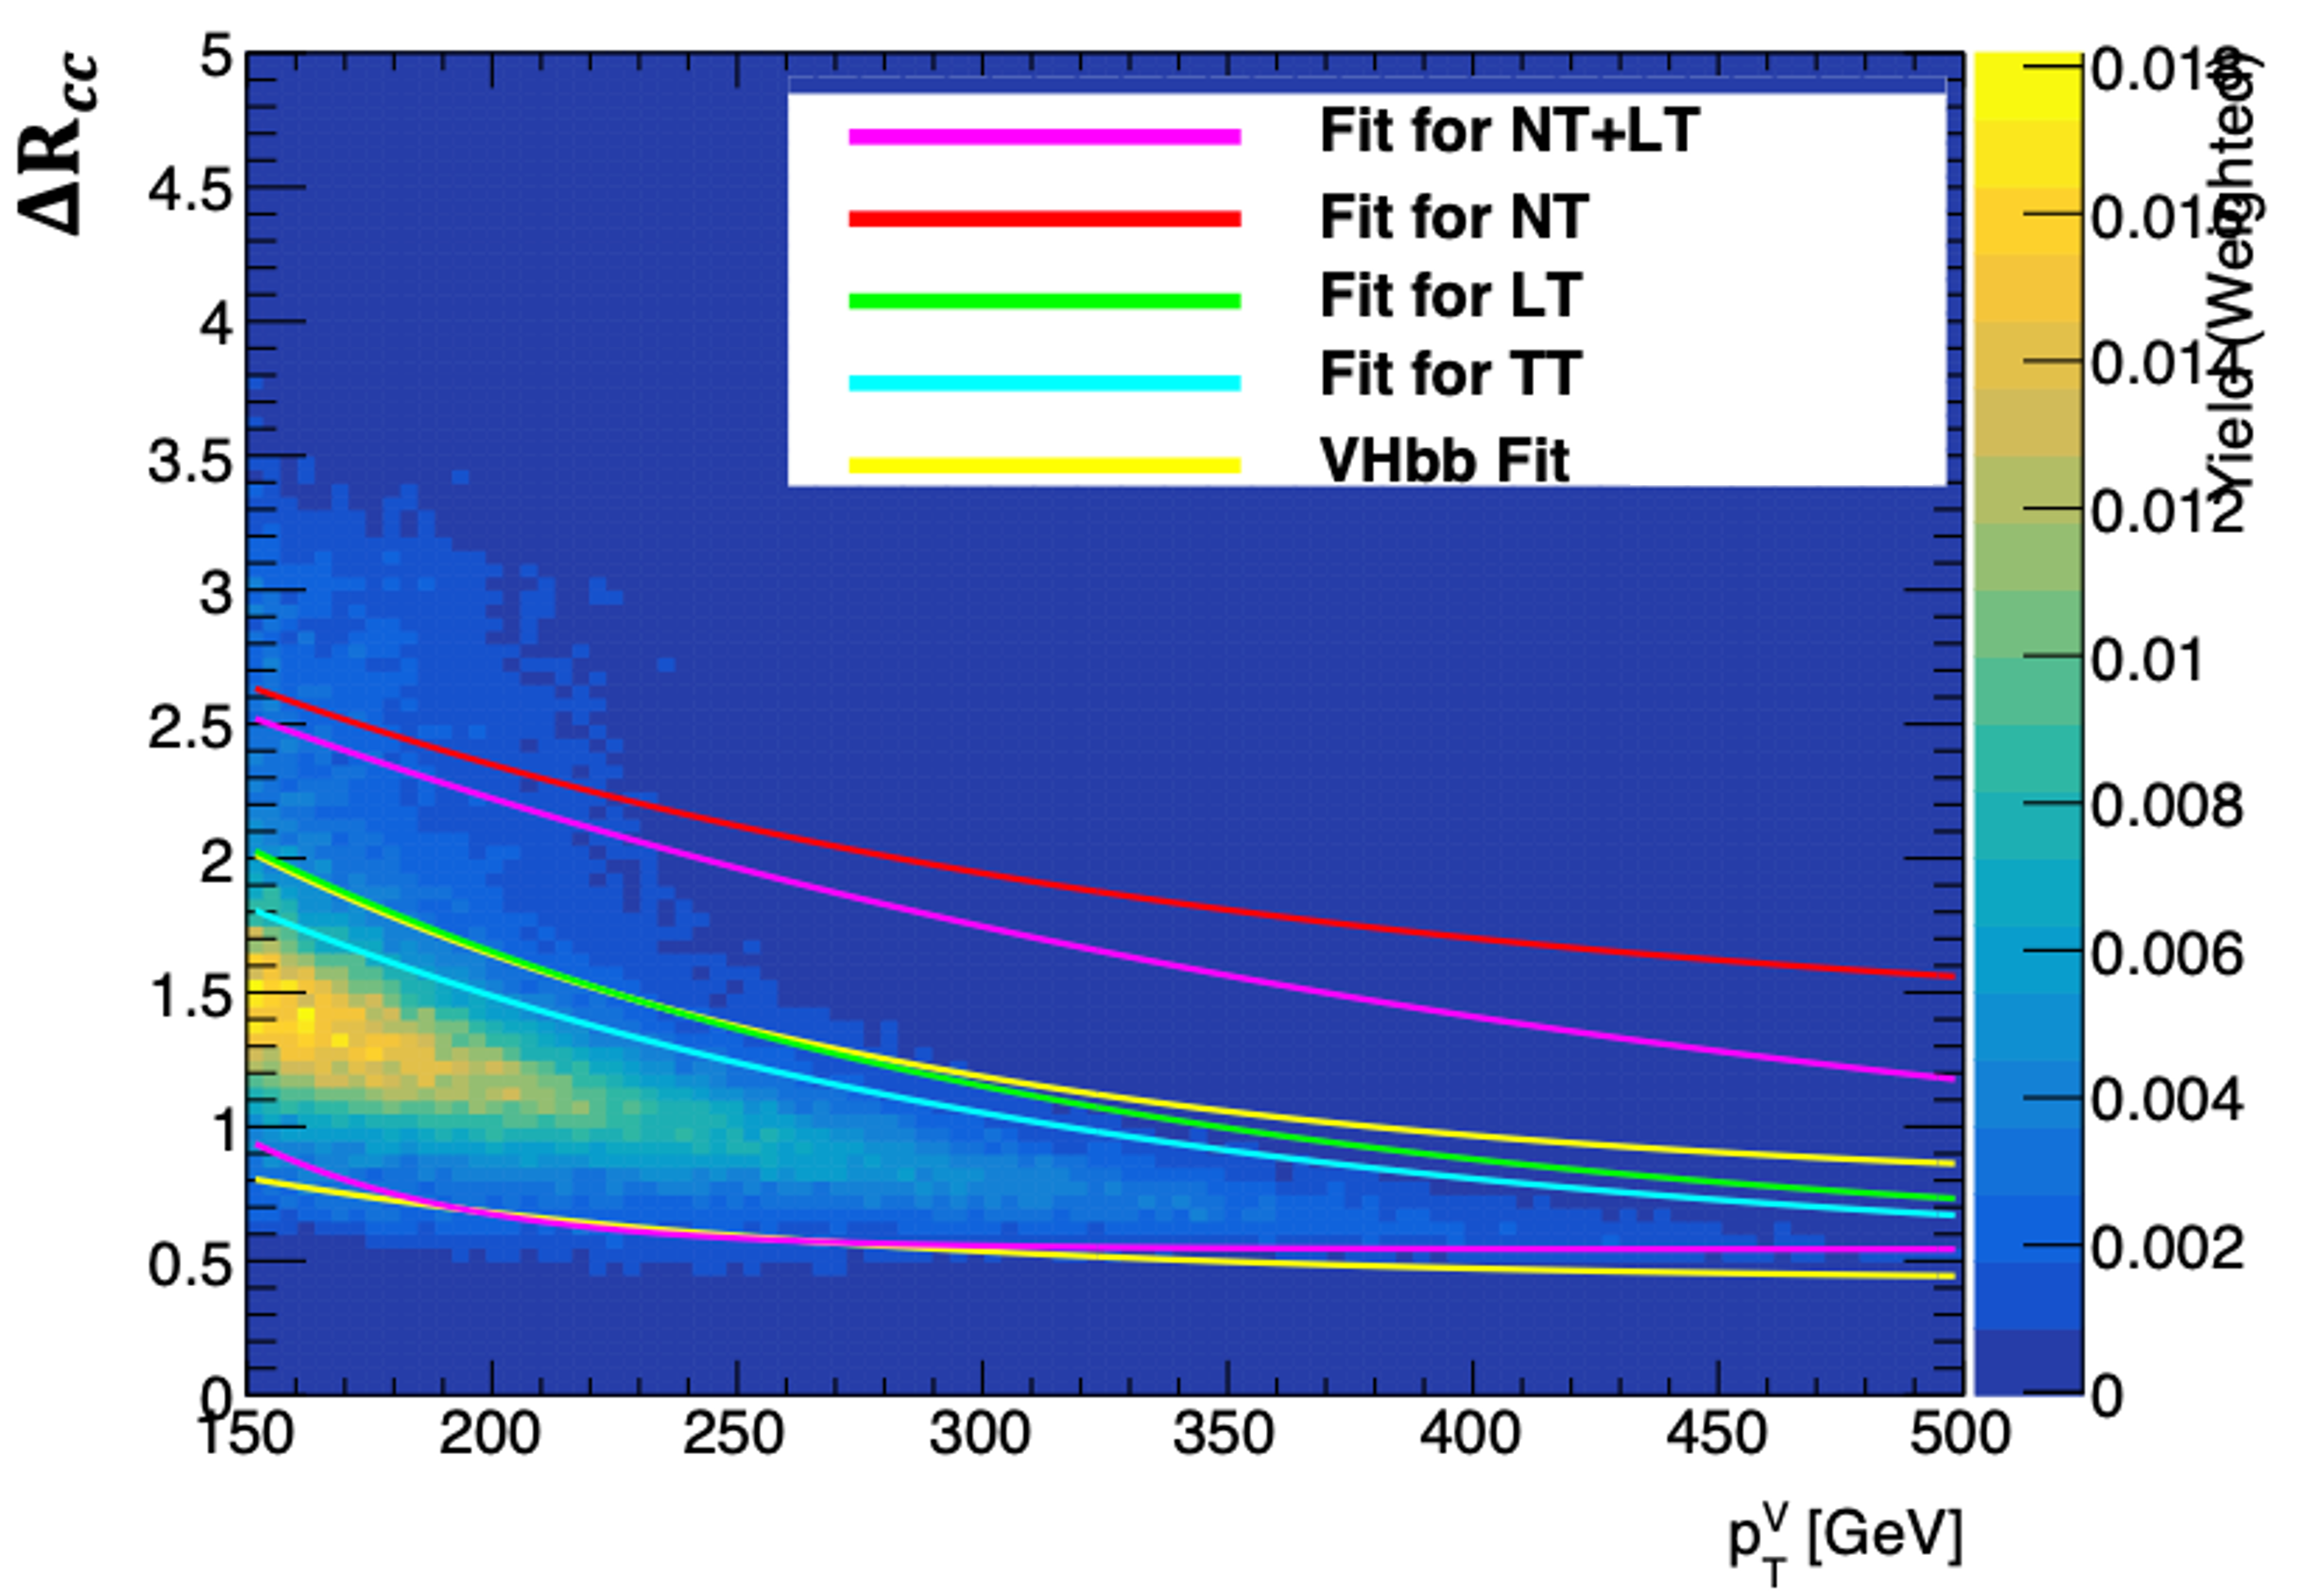
\includegraphics[width=0.48\textwidth]{Images/VH/dRccpTV/sr2.png}
    \caption{The $p_T^V$-$\Delta R_{c\bar{c}}$ 2D-histograms showing the signal yield of the 1-lepton $VH(H\rightarrow c\bar{c})$, for the 2-jet (left) and 3-jet (right) signal regions. The lines are the results of fitting the high and low $\Delta R_{c\bar{c}}-p_T^V$ cuts for various signal tags, with the yellow curve showing the $VH(H\rightarrow b\bar{b})$ $p_T^V$-$\Delta R_{b\bar{b}}$ cut.} 
    \label{fig:drccptvCutsVHcc}
\end{figure}

\begin{figure}[h!]
  \centering
  \begin{subfigure}[b]{0.32\textwidth}
      \centering
      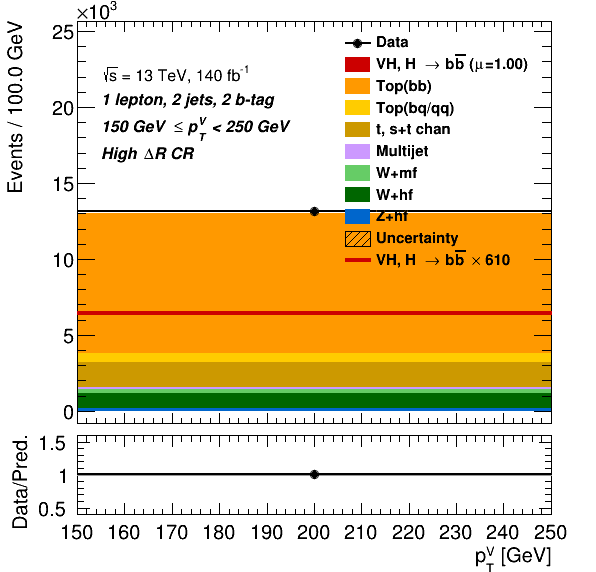
\includegraphics[width=\textwidth]{Images/VH/Own_fit/prefit_VHbb/Region_distpTV_BMax250_BMin150_DCRHigh_J2_TTypebb_T2_L1_Y6051_Prefit.png}
      \caption{1-lepton, $BB$.}
      \label{fig:plots_VHcc_ex_OL_CRH}
  \end{subfigure}
  \begin{subfigure}[b]{0.32\textwidth}
      \centering
      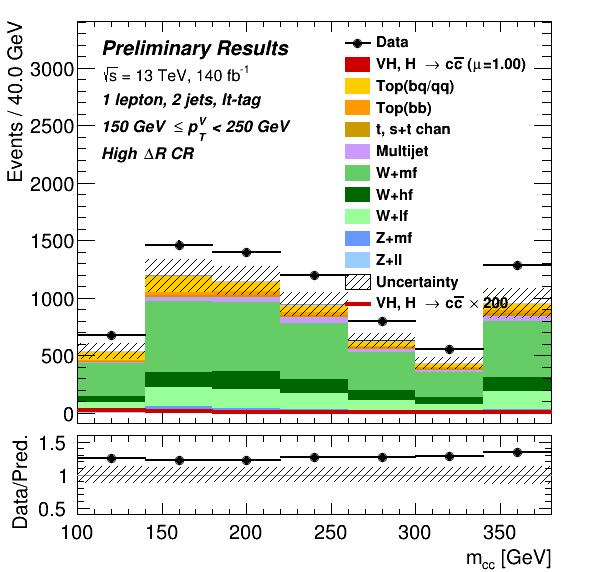
\includegraphics[width=\textwidth]{Images/VH/Own_fit/prefit_VHcc/Region_distmBB_BMax250_BMin150_DCRHigh_J2_TTypelt_T2_L1_Y6051_Prefit.png}
      \caption{1-lepton $LT$.}
      \label{fig:plots_VHcc_ex_1L_CRH}
  \end{subfigure}
  \begin{subfigure}[b]{0.32\textwidth}
    \centering
    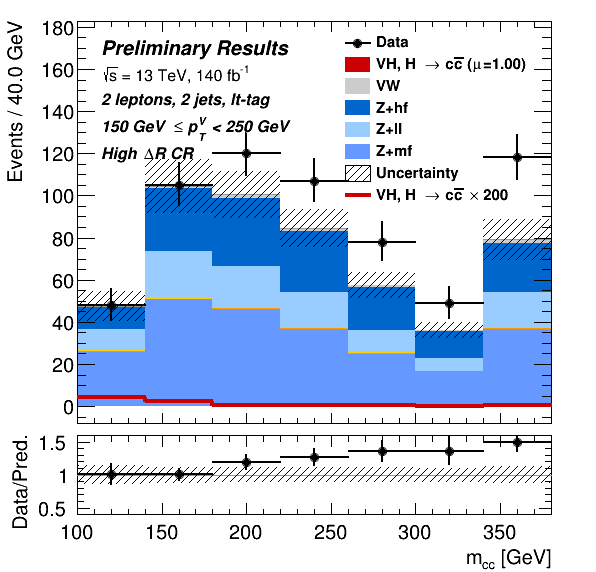
\includegraphics[width=\textwidth]{Images/VH/Own_fit/prefit_VHcc/Region_distmBB_BMax250_BMin150_DCRHigh_J2_TTypelt_T2_L2_Y6051_Prefit.png}
    \caption{2-lepton $LT$.}
    \label{fig:plots_VHcc_ex_2L_CRH}
\end{subfigure}
  \caption{Some \highdr\ \gls{cr}s (CRHigh) with 2 jets and 150 < \ptv\ < 250 GeV.}
  \label{fig:plots_VHcc_ex_CRH}
\end{figure} 

\paragraph{The Low $\Delta R$ Control region:} an extra low-$\Delta R$ control region (CRLow) is used in \vhb\ 1L to better control the $W+$hf contribution. This cut is defined similarly to the \highdr\ one with objective to let 90\% of the diboson events in the signal region, as presented in the bottom part of the plots in Figure \ref{fig:drccptvCutsVHcc}. The cuts used are defined in the right of Table \ref{tbl:CRhigh_definition}, where events with a $\Delta R$ above the cutting line enter the signal region, while those below go in the CRLow. In \vhc\ and the 0L and 1L \vhb, the CRLow is merged with the signal region as it has little impact. An example of a CRLow region is presented in the left of Figure \ref{fig:plots_VH_ex_CRL_CRvl}.

\paragraph{Top Control Regions in 0L and 1L:} they are defined to better control the Top background Top($bc$) and Top($bl$) components\footnote{The component in the parenthesis refers to the flavour of the Higgs candidates.}. The so-called \textit{Top(bc) CRs} are shared by resolved \vhb\ and \vhc, with similar \ptv\ and jet multiplicity categorisation as the \gls{sr}. In 0L and 1L, they are defined by requiring events to have at least one $B$-tag and at least one tight $c$-tag $T$, making them orthogonal to the signal regions. The Higgs candidate is reconstructed from the leading $B$ jet among $B$-tagged jet and leading $T$ jet among $T$-tagged jet, for kinematic similarity with the \gls{sr}. The Top($bb$) component, which is significant for \vhb, is controlled from the previously defined HighCRs in 0L and 1L, thanks to the large $\Delta R$ between the produced $b$ jets in a \ttb as shown in Figure \ref{fig:plots_VHcc_ex_OL_CRH}. Two examples of Top $BT$ control regions are presented in the left of Figure \ref{fig:plots_VHcc_ex_TopCR}.

\begin{figure}[h!]
  \centering
  \begin{subfigure}[b]{0.32\textwidth}
      \centering
      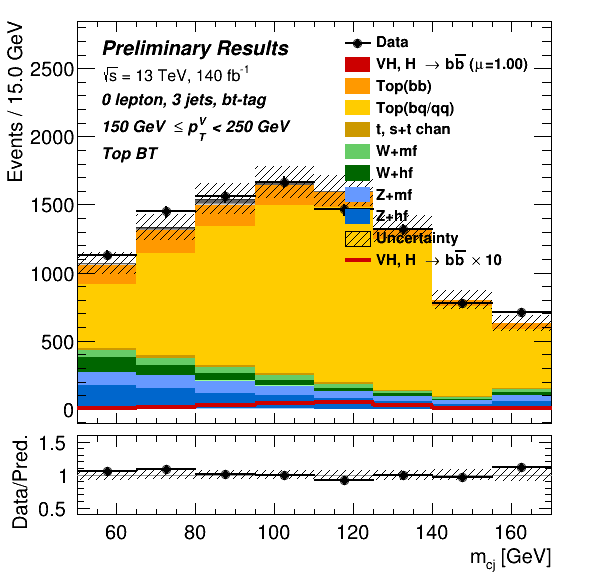
\includegraphics[width=\textwidth]{Images/VH/Own_fit/prefit_VHcc/Region_distmBB_BMax250_BMin150_DtopCRBC_J3_TTypebt_T1_L0_Y6051_Prefit.png}
      \caption{0-lepton, $BT$, 3-jet.}
      \label{fig:plots_VHcc_ex_OL_TopCR}
  \end{subfigure}
  \begin{subfigure}[b]{0.32\textwidth}
      \centering
      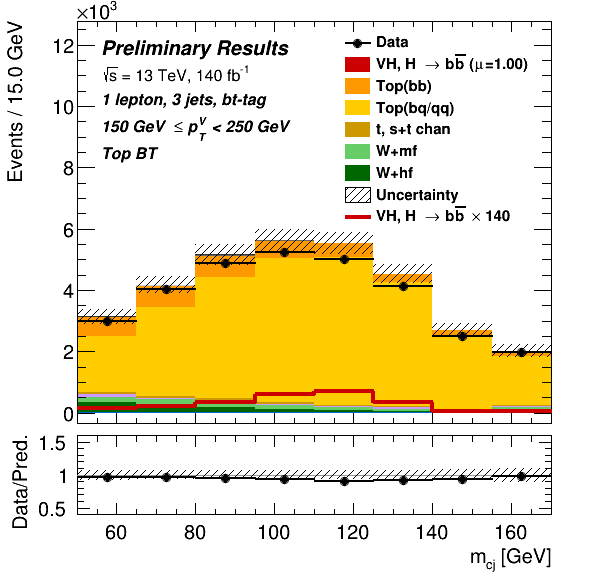
\includegraphics[width=\textwidth]{Images/VH/Own_fit/prefit_VHcc/Region_distmBB_BMax250_BMin150_DtopCRBC_J3_TTypebt_T1_L1_Y6051_Prefit.png}
      \caption{1-lepton, $BT$, 3-jet.}
      \label{fig:plots_VHcc_ex_1L_TopCR}
  \end{subfigure}
  \begin{subfigure}[b]{0.32\textwidth}
    \centering
    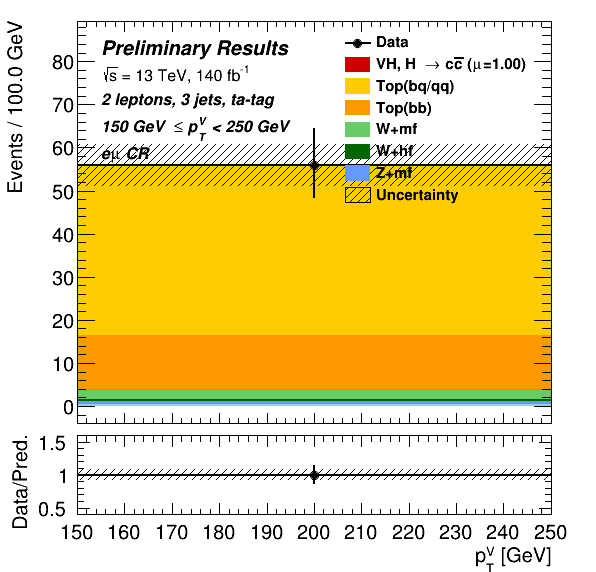
\includegraphics[width=\textwidth]{Images/VH/Own_fit/prefit_VHcc/Region_distpTV_BMax250_BMin150_Dtopemucr_J3_TTypeta_T2_L2_Y6051_Prefit.png}
    \caption{2-lepton, $e\mu$, $\geq$ 1 $T$-tag.}
    \label{fig:plots_VHcc_ex_2L_TopCR}
\end{subfigure}
  \caption{Two Top CR $BT$-tagged (left \& centre) and a Top $e\mu$CR (right), 3-jet 150 < \ptv\ < 250 GeV.}
  \label{fig:plots_VHcc_ex_TopCR}
\end{figure} 

\paragraph{Top Control Regions in 2L:} where the Top background is mostly made of di-leptonic \ttb\ decays. High purity Top \gls{cr} are derived for the 2-lepton channels by requiring leptons of different flavours ($e\mu$ or $\mu e$) instead of the same flavour ($ee$ or $\mu\mu$). These so-called \textit{Top} $e\mu$ \textit{CRs} are used to derive a \ttb\ background template in a data-driven way for the \gls{sr}s in \vhb. For \vhc, the \ttb\ is a less significant component due to the tagging requirement and the $e\mu$ enters the fit as a standard \gls{cr} per \ptv\ and jet multiplicity, with at least one $T$-tag. An example of such a \gls{cr} is presented in Figure \ref{fig:plots_VHcc_ex_2L_TopCR}.

\paragraph{$V +$light-jet Control Regions:} is particularly significant for \vhc, due to the difficulties in discriminating $c$-jets from light- and $b$-jets. Dedicated \gls{cr} in 1L and 2L for the $W+l$ and $Z+l$ backgrounds respectively are defined by requiring exactly one loose $L$-tag without any $T$- nor $B$-tagged jet in the event. The selection is otherwise similar to that of the signal region, with the candidate pair now tagged as $LN$, with $N$ being the leading untagged jet. The 1L $V+l$ \gls{cr} obtains a purity of 60\% of $W+l$, while the 2L $V+l$ reaches a purity of $Z+l$ of 70\%.

\begin{figure}[h!]
  \centering
  \begin{subfigure}[b]{0.32\textwidth}
      \centering
      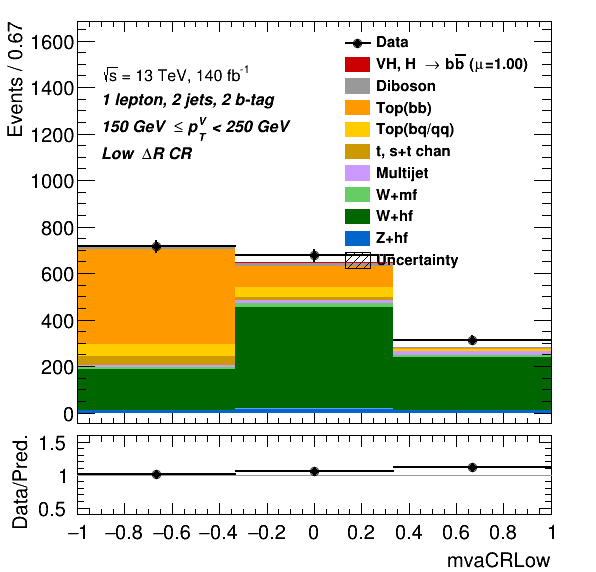
\includegraphics[width=\textwidth]{Images/VH/Own_fit/prefit_VHbb/Region_distmvaCRLow_BMax250_BMin150_DCRLow_J2_TTypebb_T2_L1_Y6051_Prefit.png}
      \caption{1-lepton \lowdr\ CR, $BB$.}
      \label{fig:plots_VHb_ex_1L_CRL}
  \end{subfigure}
  \begin{subfigure}[b]{0.32\textwidth}
      \centering
      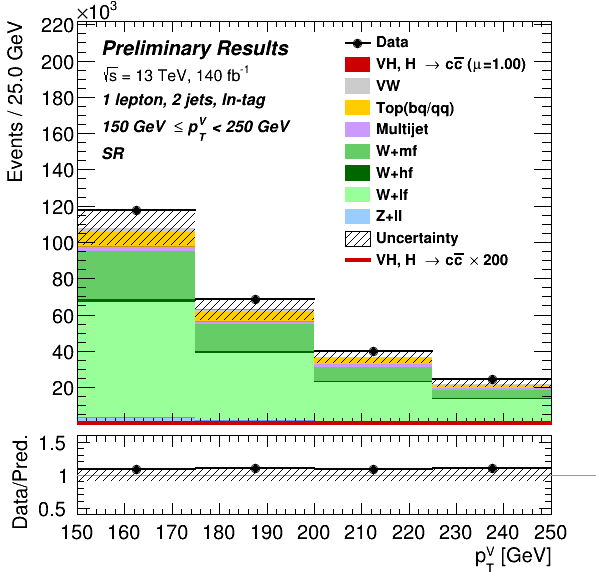
\includegraphics[width=\textwidth]{Images/VH/Own_fit/prefit_VHcc/Region_distpTV_BMax250_BMin150_DSR_J2_TTypeln_T1_L1_Y6051_Prefit.png}
      \caption{1-lepton $V+l$ CR $LN$.}
      \label{fig:plots_VHcc_ex_1L_CRvl}
  \end{subfigure}
  \begin{subfigure}[b]{0.32\textwidth}
    \centering
    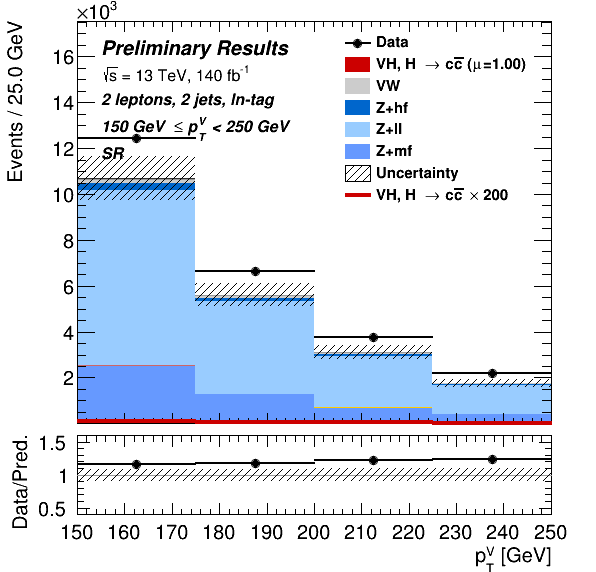
\includegraphics[width=\textwidth]{Images/VH/Own_fit/prefit_VHcc/Region_distpTV_BMax250_BMin150_DSR_J2_TTypeln_T1_L2_Y6051_Prefit.png}
    \caption{2-lepton $V+l$ CR $LN$.}
    \label{fig:plots_VHcc_ex_2L_CRvl}
\end{subfigure}
  \caption{A $BB$-tagged \lowdr\ CR (left) and two $LN$-tagged $V+l$ CRs (centre \& right), both in 2 jets 150 < \ptv\ < 250 GeV.}
  \label{fig:plots_VH_ex_CRL_CRvl}
\end{figure} 

\subsubsection{Boosted Regime Categorisation}
In the boosted \vhb, two \ptv\ bins are defined above 400 GeV to avoid overlap with the resolved \vhb: [400, 600] GeV and $\geq$ 600 GeV. The \gls{sr}s are defined by requiring exactly two of the three leading subjets associated to a single learding large-$R$ jet to be $b$-tagged, with no additional jet outside the large-$R$ jet being $B$-tagged to enhance the top background rejection. The \gls{sr}s are further split into a \textit{high-purity signal region} (HP SR) and a \textit{low-purity signal region} (LP SR) depending on the number of small-$R$ jets outside the large-$R$ jet. All boosted regions are presented in Appendix \ref{appsec-vh-analRegBoo}. 

\begin{figure}[h!]
  \centering
  \begin{subfigure}[b]{0.32\textwidth}
      \centering
      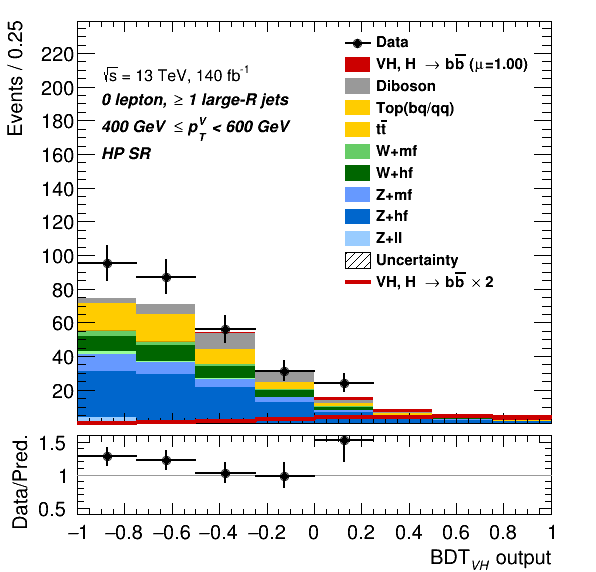
\includegraphics[width=\textwidth]{Images/VH/Own_fit/prefit_VHbb/Region_distmva_BMax600_BMin400_incFat1_Fat1_DSRnoaddbjetsr_J0_TTypebb_T2_L0_Y6051_Prefit.png}
      \caption{0-lepton high purity SR.}
      \label{fig:plots_VHboost_ex_0L_SR}
  \end{subfigure}
  \begin{subfigure}[b]{0.32\textwidth}
      \centering
      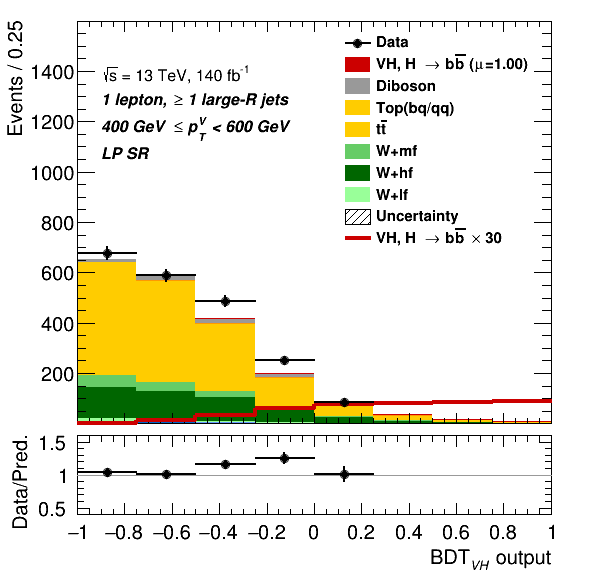
\includegraphics[width=\textwidth]{Images/VH/Own_fit/prefit_VHbb/Region_distmva_BMax600_BMin400_incFat1_Fat1_DSRnoaddbjetsr_J1_TTypebb_incJet1_T2_L1_Y6051_Prefit.png}
      \caption{1-lepton low purity SR.}
      \label{fig:plots_VHboost_ex_1L_SR}
  \end{subfigure}
  \begin{subfigure}[b]{0.32\textwidth}
    \centering
    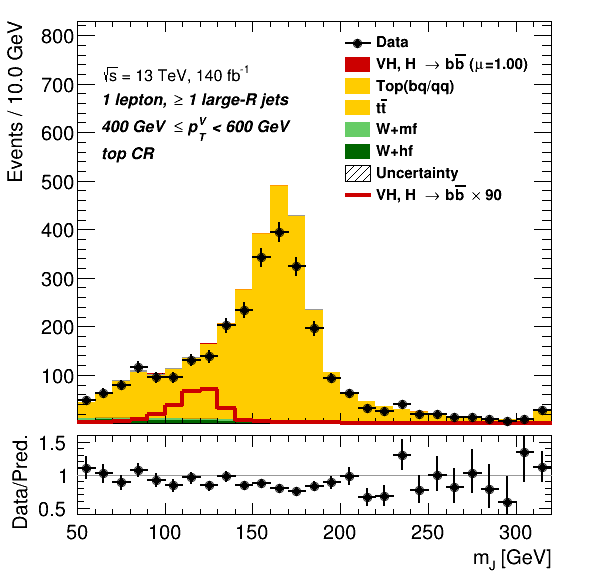
\includegraphics[width=\textwidth]{Images/VH/Own_fit/prefit_VHbb/Region_distmBB_BMax600_BMin400_incFat1_Fat1_DSRtopaddbjetcr_J0_TTypebb_incJet1_T2_L1_Y6051_Prefit.png}
    \caption{1-lepton top CR.}
    \label{fig:plots_VHboost_ex_1L_top}
\end{subfigure}
  \caption{Some boosted $BB$-tagged with 400 < \ptv\ < 600 GeV regions signal regions (left \& centre) and boosted Top CR (right).}
  \label{fig:plots_VHboost_ex}
\end{figure} 

\paragraph{Boosted Top Control Regions in 0L and 1L}: events that have an additional $B$-tagged track-jet outside the large-$R$ jet as defined by an angular separation of $\Delta R(\textrm{VR-track jet, large-}R\textrm{ jet}) > 1$
define the boosted Top control regions in 0L and 1L. The \ttb\ background is the main background in these lepton channels, when a $t$ decay is capture as a single large-$R$ jet merging the produced $b$ and a hadronically decaying $W$. The boosted TopCR effectively captures this process by identifying the $b$-quark from the other decay $t$-quark in the \ttb\ pair with the same 85\% \gls{wp}.\\

\newpage

\begin{sidewaysfigure}[t!]
    \centering
    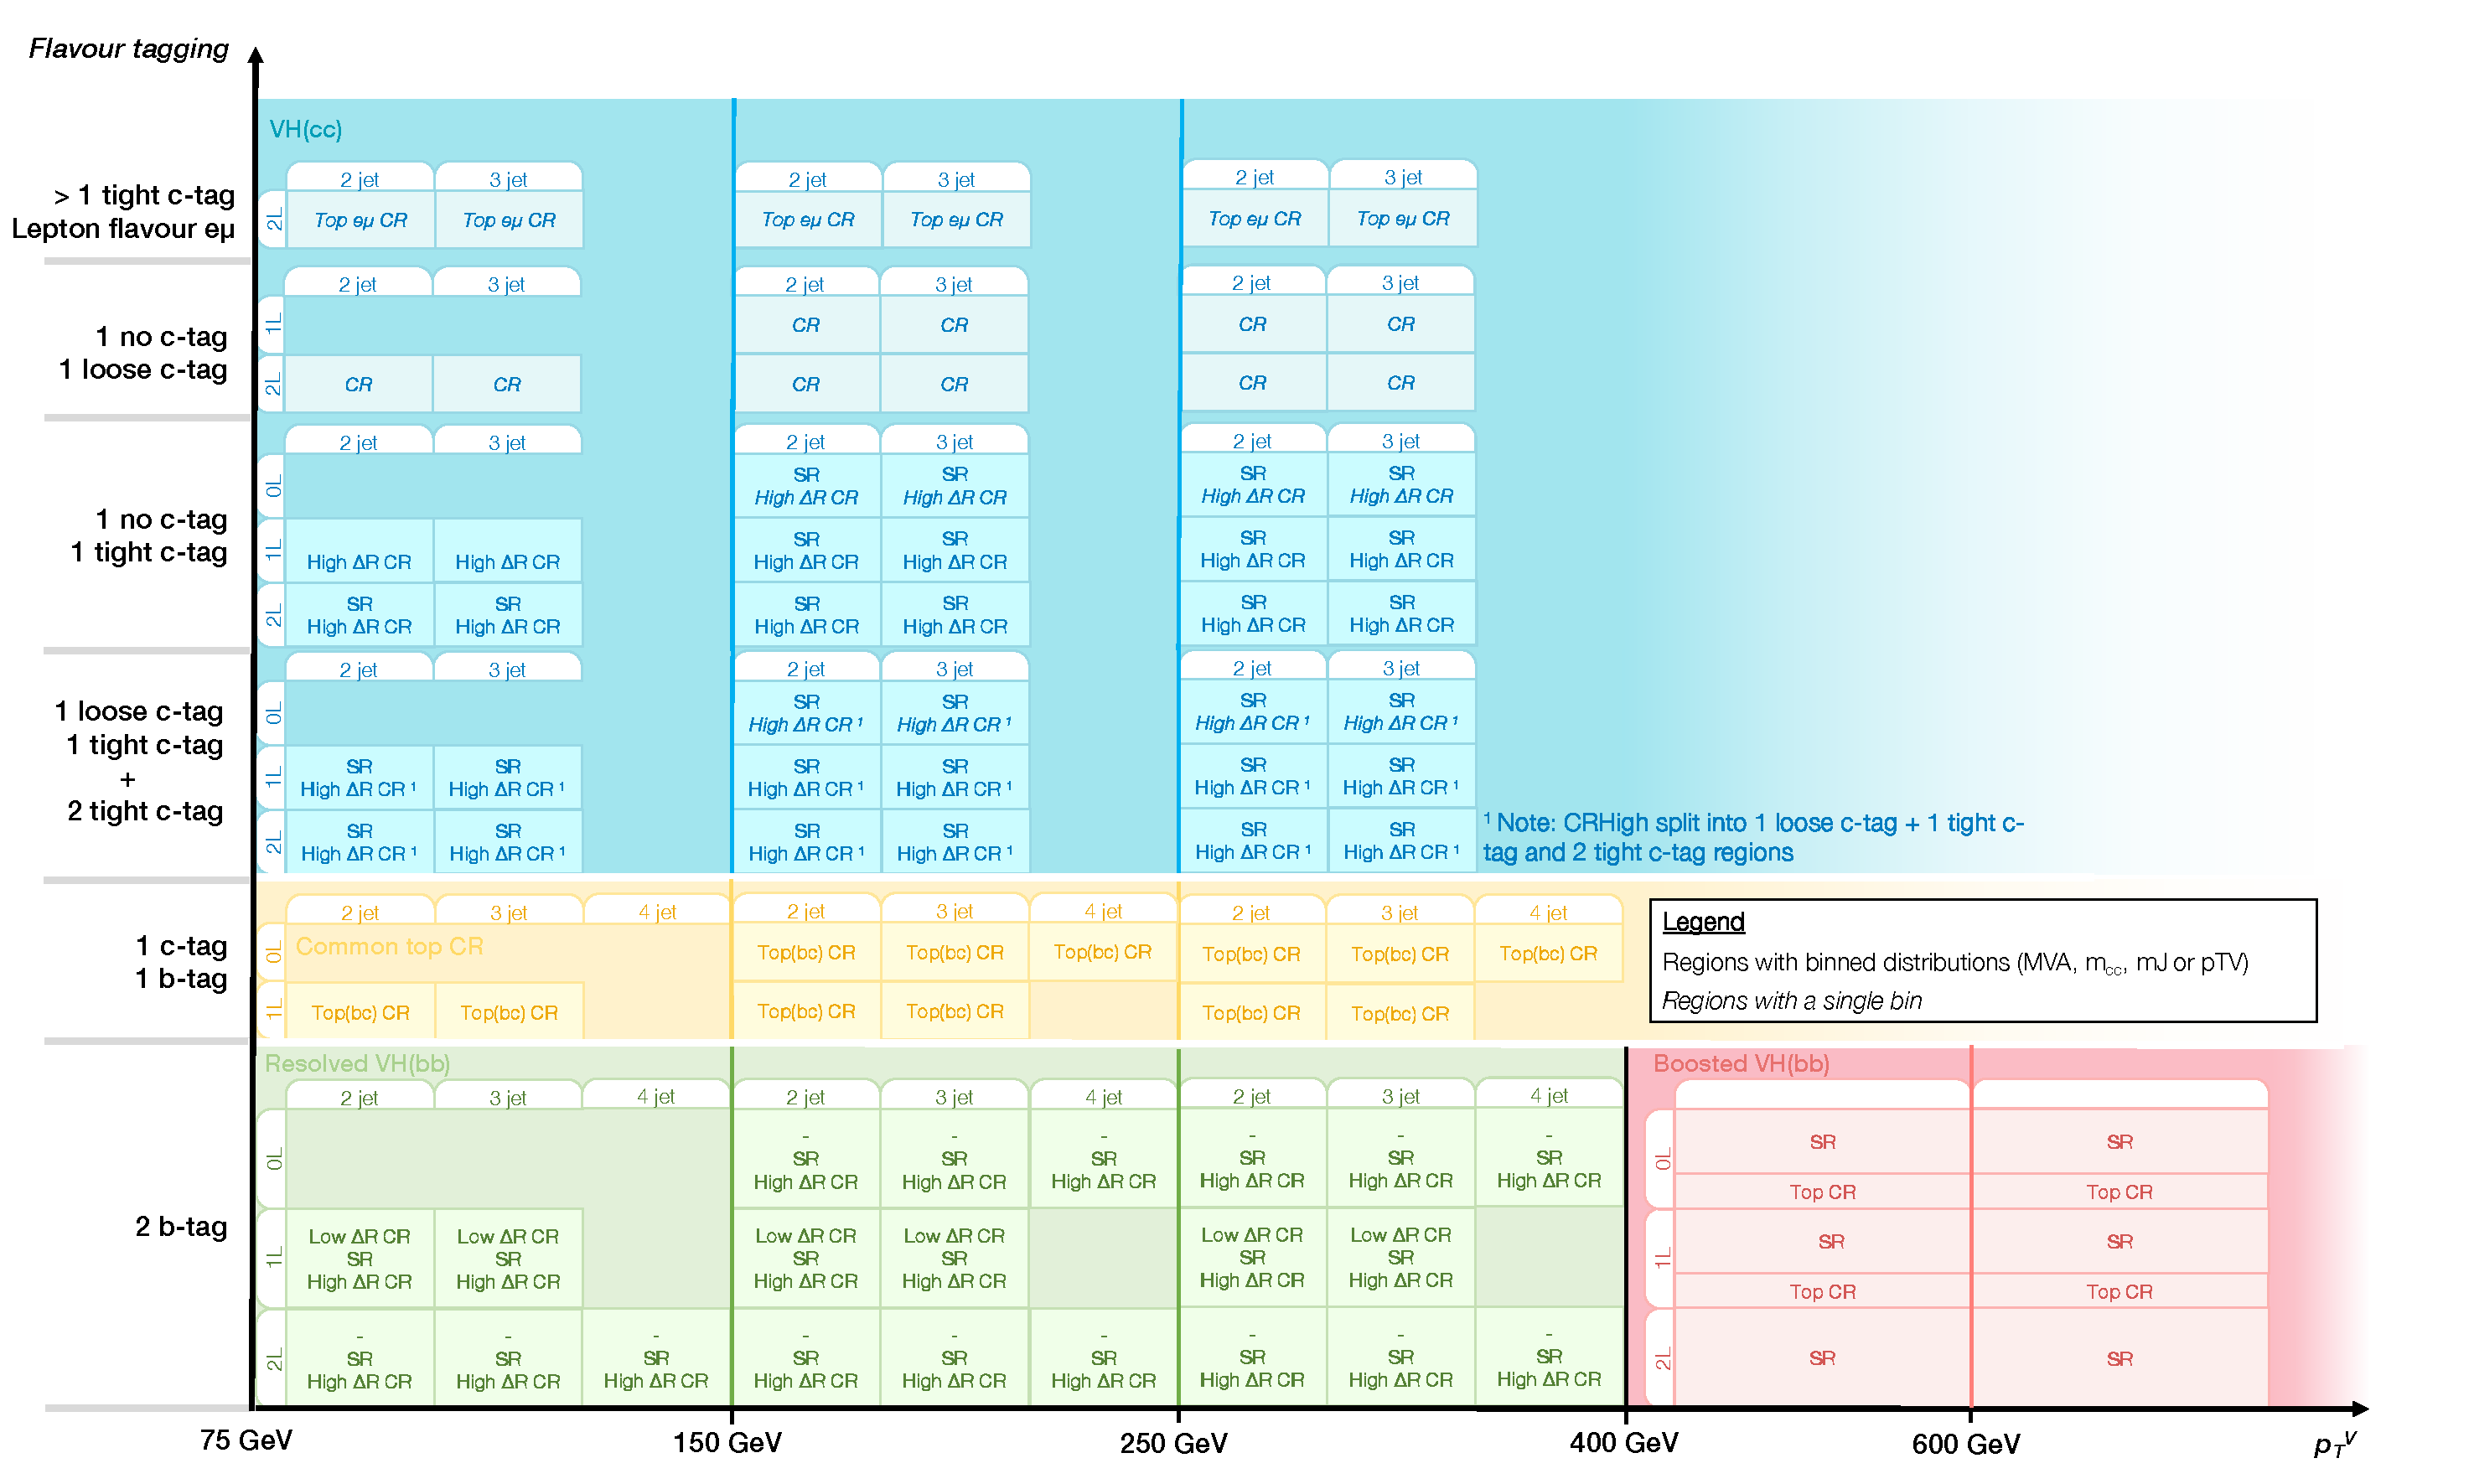
\includegraphics[width=\textwidth]{Images/VH/Cat/VH_analysis_cat.pdf}
    \caption{The current split of the analysis regions considered in the $VH (H\rightarrow b\bar{b}/c\bar{c})$ Combined Analysis, showing the Signal Region (SR), High and Low $\Delta R$ control region (CR), and the Top CR. From the internal documentation.} 
    \label{fig:ana-strat-det}
\end{sidewaysfigure}

\clearpage

\subsection{Truth Tagging}
The tagging method described in Section \ref{sec-selectionandcat}, referred to as \textit{direct tagging}, is a cut-based method where a jet passes or fails a threshold cut, as defined by dedicated working points in the \gls{pcft} or PCBT schemes. These \gls{wp} have a large rejection for $b$-tagging due to the good performance of the method. For $c$-jets, the tagging efficiency is low and many $c$-jets end up rejected by the selection. This problem is compounded by the event selection criteria, requiring two $b$-tags or at least one tight $c$-tag to enter the analysis' regions. Only a part of the events in the simulated samples satisfy these requirements, and most are discarded from the analysis. Having sufficient \gls{mc} statistics in all regions is essential to effectively model the backgrounds and reduce the \gls{mc} statistical uncertainty. An alternative approach to direct tagging used in the analysis to retain the large \gls{mc} statistics is \textit{truth tagging}. Rather than applying a pass-fail decision, truth tagging reweighs events by their probability of being selected at a specific working point, based on truth information only available in the simulated samples. The tagging scale factors are applied in the analysis after truth tagging. \\

Mathematically, truth tagging derives a per event weight $w$ from the tagging efficiency $\epsilon_j(\textbf{x}, \theta)$ for a given flavour jet $j$ to be tagged at a given working point of a classifier trained on a set of input variables $\textbf{x}$, with the assumption that the efficiency is parametrisable as a function of several variables $\theta$, such as the jet $p_T$, $\eta$, ... For a set of $m$ jets with a tagged subset $T_i$ of cardinality $|T_i| = n$, and defining the efficiency at tagging the tagged jets as \[\epsilon(T_i,\textbf{x},\theta) = \prod_{j\in T_i} \epsilon_j(\textbf{x},\theta),\] and the efficiency at not tagging the set of untagged jets $\tilde{T}$, with $|\tilde{T}_i| = m-n$, \[ \epsilon_{in}(\tilde{T}_i,\textbf{x}, \theta) = \prod_{j\in \tilde{T}_i} (1-\epsilon_j(\textbf{x}, \theta)),\] the expression for $w$ can be factorised as \cite{ATL-PHYS-PUB-2022-041}: 

\begin{equation}
  \label{eq:truthtagging1}
      w = \sum_i^C \epsilon(T_i,\textbf{x},\theta)\cdot \epsilon_{in}(\tilde{T}_i,\textbf{x},\theta),
  \end{equation}
where the sum is over all possible permutations of tags $C$. The probability of a specific configuration $i$ is given by \[ P_i = \frac{ \epsilon(T_i,\textbf{x},\theta)\cdot \epsilon_{in}(\tilde{T}_i,\textbf{x},\theta)}{w}.\] When deploying the technique, one possible permutation is randomly sampled to keep distinct bins uncorrelated in the fit and the whole weight $w$ is applied to it. \\

Technically, truth tagging was deployed with map-based 2D histograms $p_T - \eta$ parametrising the tagging efficiency of the jets in the latest standalone \vhb\ and \vhc\ analysis \cite{ATLAS:2020fcp, Collaboration:2721696}. Such histograms are called \textit{efficiency map}, leading to the implementation being referred to \textit{map-based truth tagging}. These maps were derived individually for each $b$-, $c$-, light-, and $\tau$-jets flavour and each working point. A further possibility is to combine direct tagging with truth tagging into the so-called \textit{hybrid tagging} strategy, in which a portion of the events are direct tagged and the rest is truth tagged. This last approach limits the mis-modelling incurred by truth tagging and remove the need to correct for non-closure effects. \\

A new approach considered for the combined analysis relies on a \gls{gnn} to perform the so-called \textit{GNN truth tagging} \cite{ATL-PHYS-PUB-2022-041}. This removes the statistical dispersion limitation of high-dimension efficiency maps. Interestingly, it also becomes possible to include more variables to parametrise the efficiency, leading to better agreement with the direct tagging distribution comparing to map-based truth tagging. The network builds a fully-connected graph with several layers message-passing updates \cite{graphInductiveBias}, where each node represents a jet in the event\footnote{Only central jets in the resolved regime and track-jets associated with the large-$R$ jet in the boosted regime.}. The features per node are the jet-level and event-level variables listed in Table~\ref{tbl:gnn-features}, with the angular separation between the jets set as edge between the nodes. Finally, a fully-connected \gls{nn} receives the last update graph and outputs all track-jets or jets flavour-tagging efficiencies.

\begin{table}[tbp]
  \begin{center}
      \begin{tabular}{C{8cm}C{5cm}} \hline \hline
        Jet features & Type of variable \\ 
        \hline
        Jet $p_T$ & \\
        Jet $\eta$ & \\
        Jet $\phi$ & \\
        Jet flavour label & Jet level feature \\
        Mass of $p_T$ leading b or c hadron in the jet $\phi$ & \\
        $p_T$ of $p_T$ leading b or c hadron in the jet $\phi$ & \\
        $\eta$ of $p_T$ leading b or c hadron in the jet $\phi$ & \\
        $\phi$ of $p_T$ leading b or c hadron in the jet $\phi$ & \\
        \hline
        Average number of interactions per event $\langle \mu \rangle$ & Event level variable\\
        \hline
        Angular separation between two jets $\Delta R$ & Jet-pair variable\\
        \hline \hline
      \end{tabular}
    \caption{The input features to parametrise the efficiency in GNN truth tagging.}
    \label{tbl:gnn-features}
  \end{center}
\end{table}

In the combined analysis, truth tagging is deployed in all regimes and trained independently for samples with different \gls{mc} generators\footnote{Since the \glsfirst{sf} are derived per generator.}, inclusively in all lepton channels. In the resolved regime, the training is further separated for each background samples. The GNN truth tagging is seen to improve the parametrisation of the efficiency, showing better closure with the direct-tagged distributions than the map-based approach. However, some unclosure remain for particular flavours. To limit this effect, hybrid tagging is also deployed in the combined analysis with GNN truth tagging. In this hybrid tagging, $b$-jets are direct tagged and other jets are GNN truth tagged in the resolved regime. In the boosted regime, all jets are truth tagged due to the limited \gls{mc} statistics. The strategies deployed in the different regimes of the analysis are summarised in Table \ref{tbl:gnn-strategy}.

\begin{table}[!htbp]
  \begin{center}
      \begin{tabular}{c|c|c|c} \hline \hline
        & \vhb\ Resolved & \vhc\ & \vhb\ Boosted\\ 
        \hline
        Hybrid tagging & Yes ($b$-jets are DT) & No (fully TT) & No (fully TT)  \\
        Truth tag \gls{wp} & 70\% $b$ \& 70\% $b$ & $c$-tight \& $c$-tight & 85\% $b$ \& 85\% $b$ \\
        MC stat. \% for TT regions & 100\% & 8\% & 100\%\\
        \hline
        $V+$jets & HT & TT & TT\\
        single-top $s/t$ & HT & TT & TT\\
        single-top $Wt$ & DT & DT & TT\\
        \ttb\ & DT & DT & TT\\
        diboson & DT & DT & TT\\
        signal & DT & DT & DT\\
        \hline \hline
      \end{tabular}
    \caption{The tagging strategies to be used in the different regimes of the analysis, with truth tagging (TT), direct tagging (DT), and hybrid tagging (HT).}
    \label{tbl:gnn-strategy}
  \end{center}
\end{table}

The tagging strategy is optimised to maximise the \gls{mc} statistics of the different regions and boost the sensitivity. Truth and hybrid tagging are only deployed when they deliver a meaningful improvement to the analysis. The full tagging strategy of the analysis is:
\begin{itemize}
  \item Resolved \vhb: direct tagging is used except for the $V+$jets and single-top $s/t$ process where hybrid tagging is deployed, with both $b$-jets being direct tagged at the 70\% \gls{wp}.
  \item \vhc: similar to the resolved \vhb, with the $V+$jets and single-top $s/t$ now fully GNN truth tagged. For \vhc, the samples are split based on the tag region to avoid reusing an event twice. For example, an initially $LN$ direct-tagged event could enter the $TT$ region with a low truth tag weight, thereby removing the statistical independence assumed between \gls{mc} events. To correct this, only 8\% of the \gls{mc} statistics is randomly sampled and truth tagged to the $TT$-tag region, and the rest is passed to direct tagging (for the $TL$, $NT$, $LN$, and $BT$ tags). 
  \item Boosted \vhb: GNN truth tagging is applied for all background except the signal samples that are direct tagged.
\end{itemize}
Unfortunately, at the time of writing this thesis the analysis samples were not yet fully updated to the tagging scheme described here. Instead, the resolved \vhbc all use direct tagging everywhere and the boosted regime uses full GNN truth tagging. Moving to the full tagging scheme outlined above should have a small positive effect on \gls{mc} statistics uncertainty and bring smoother \gls{mc} templates, reducing the noise in the fit.
% TODO: this is not true: the main note was including this only for truth tagging, not for the rest: The above outlined strategy outlines the final strategy. The plots and yield tables - and correspondingly fit results - do not reflect this strategy yet and instead direct tagging is used for resolved \vhbb and \vhcc regimes and full GNN truth tagging for the boosted \vhbb regime, since fit inputs were not ready in time for this version of the note. The expected differences on the sensitivity are small (small decrease in the impact of MC stat. uncertainty and smoother MC templates that will make the fit less prone to statistical ``noise'' making the fit more robust.)}

To showcase the effectiveness of the method, the direct tagged, GNN truth tagged, and map-based truth tagged $m_{cc}$ distributions of the \textsc{Sherpa} 2.2.11 simulated $W+$jets in the 1-lepton 2-jet CRHigh \ptv\ $\in [250, 400]$ GeV region of the \vhc\ is displayed in Figure \ref{fig:truthtaggingW1LVHcc}. The GNN truth tagging is found to be in better agreement with the direct tagged distributions in the regions of sufficient statistics. In the $W+l$ region, direct tagging leads to statistically depleted regions with large uncertainties: this is effectively corrected by the GNN-based truth tagging approach. No significant non-closures are observed for from GNN truth tagging with the outlined strategy.

\begin{figure}[h!]
  \begin{subfigure}[b]{0.32\textwidth}
    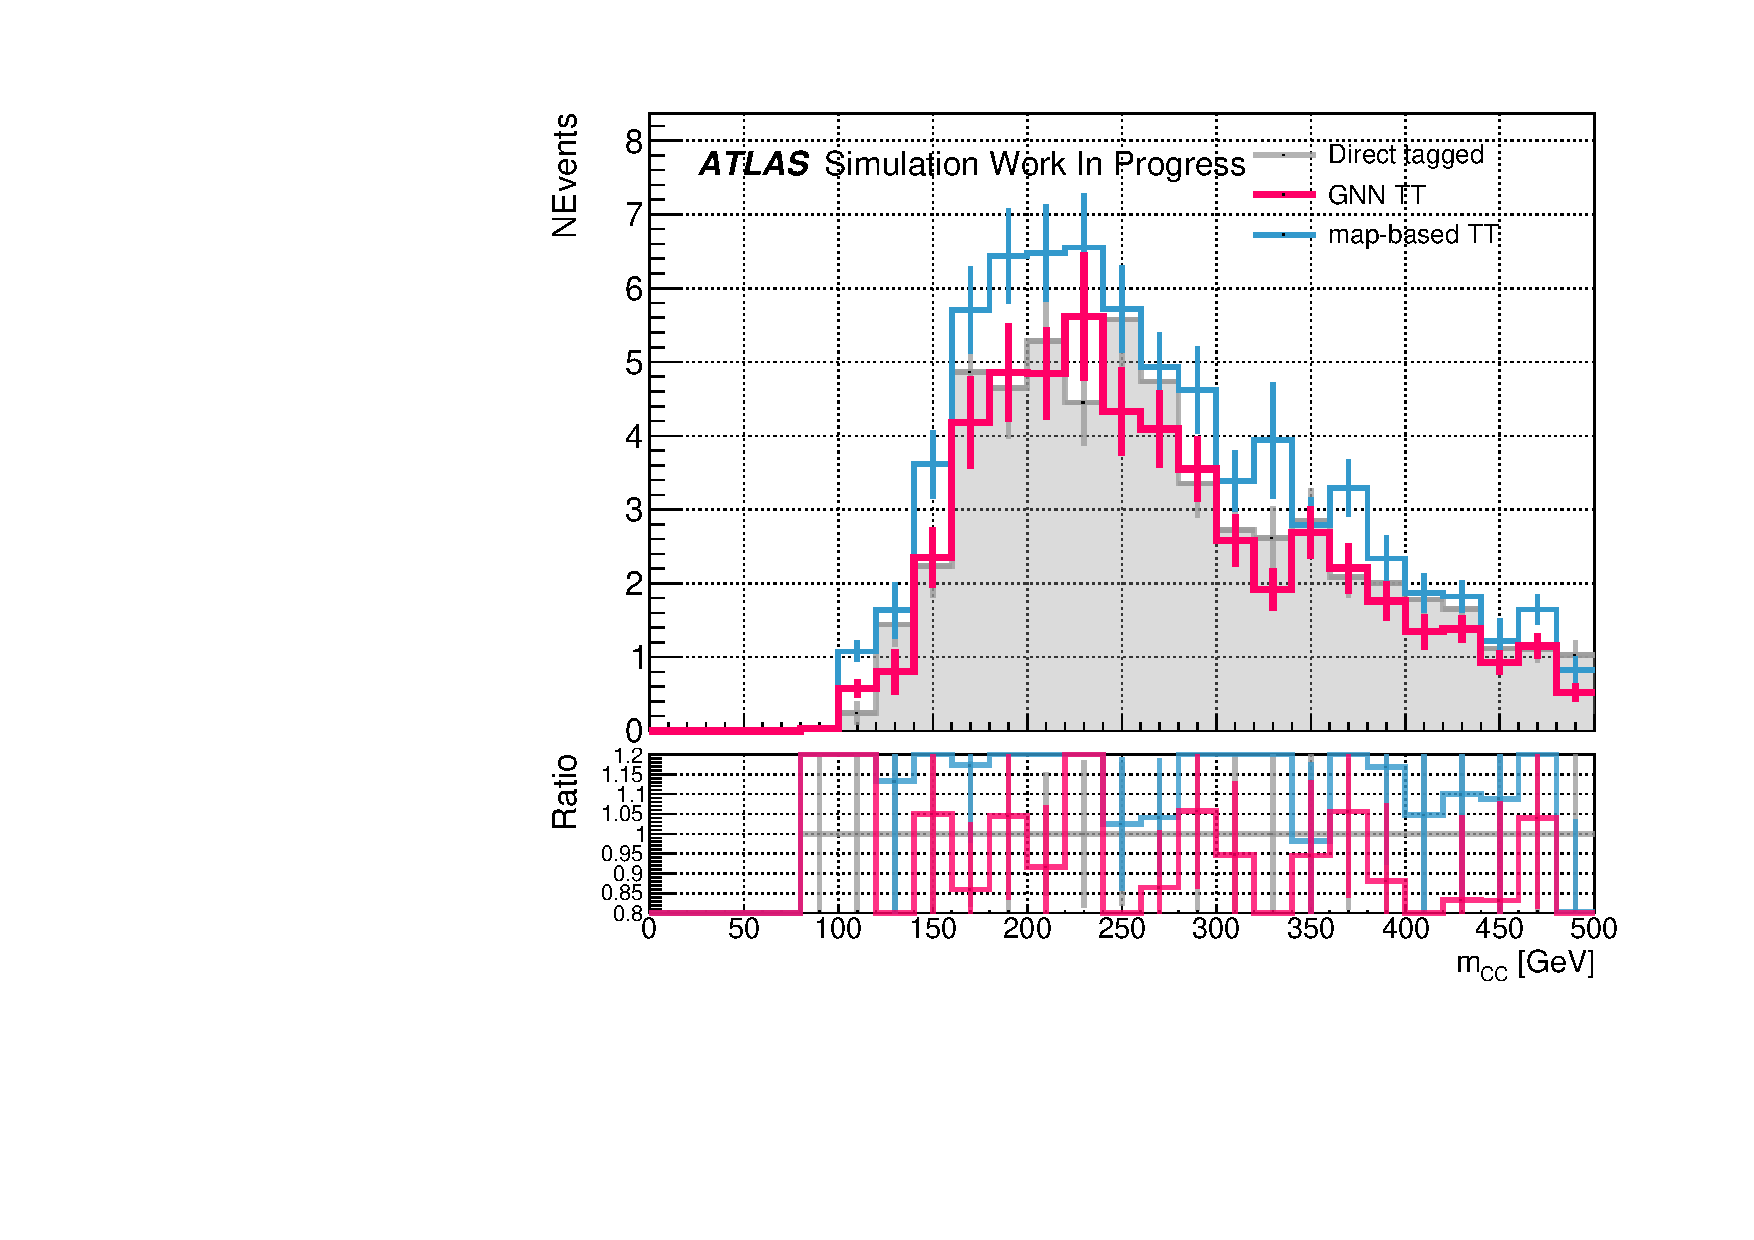
\includegraphics[width=\textwidth]{Images/VH/Tagging/Whf_2tttag2jet_250_400ptv_CRHigh_mCC.pdf}
  \caption{$W+$hf in CRHigh.} 
  \end{subfigure}
  \begin{subfigure}[b]{0.32\textwidth}
    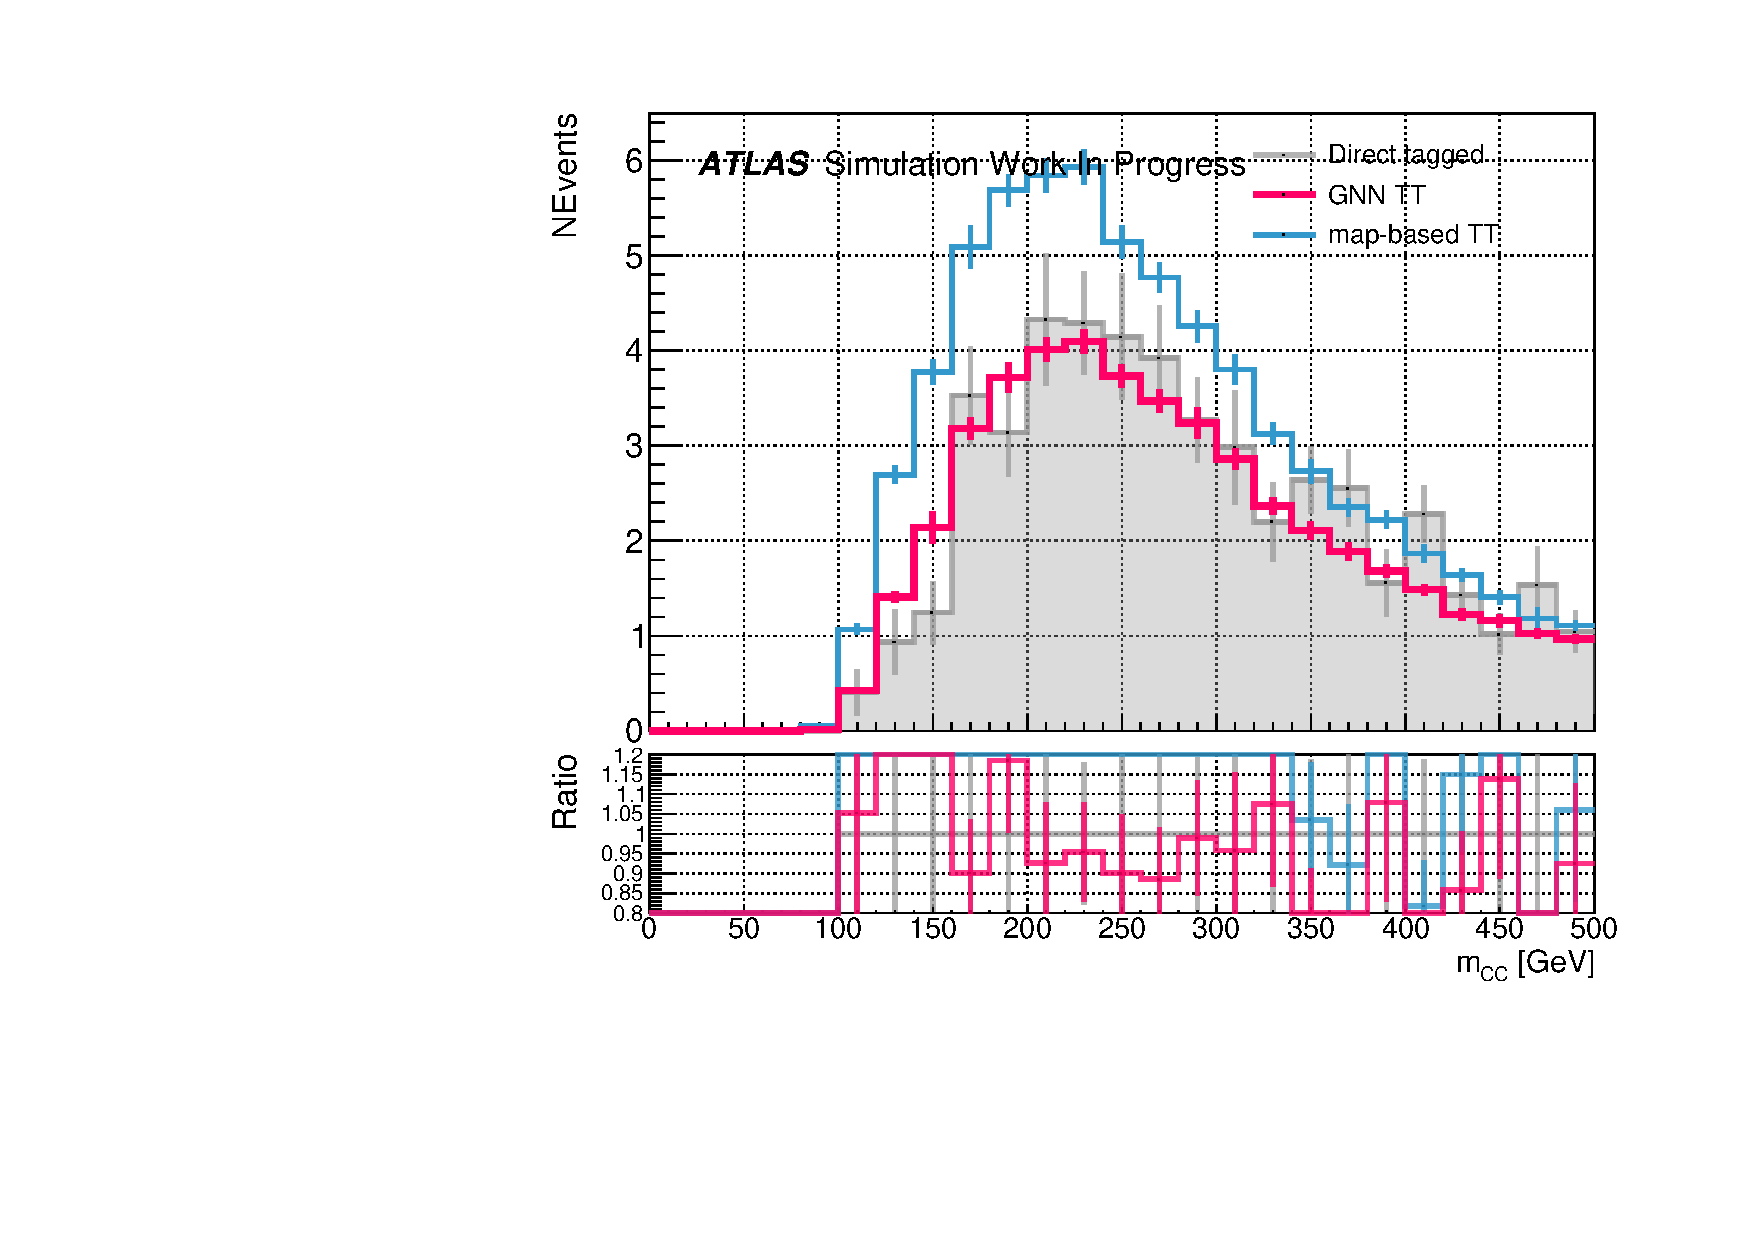
\includegraphics[width=\textwidth]{Images/VH/Tagging/Wmf_2tttag2jet_250_400ptv_CRHigh_mCC.pdf}
    \caption{$W+$mf in CRHigh.}
  \end{subfigure}
  \begin{subfigure}[b]{0.32\textwidth}
    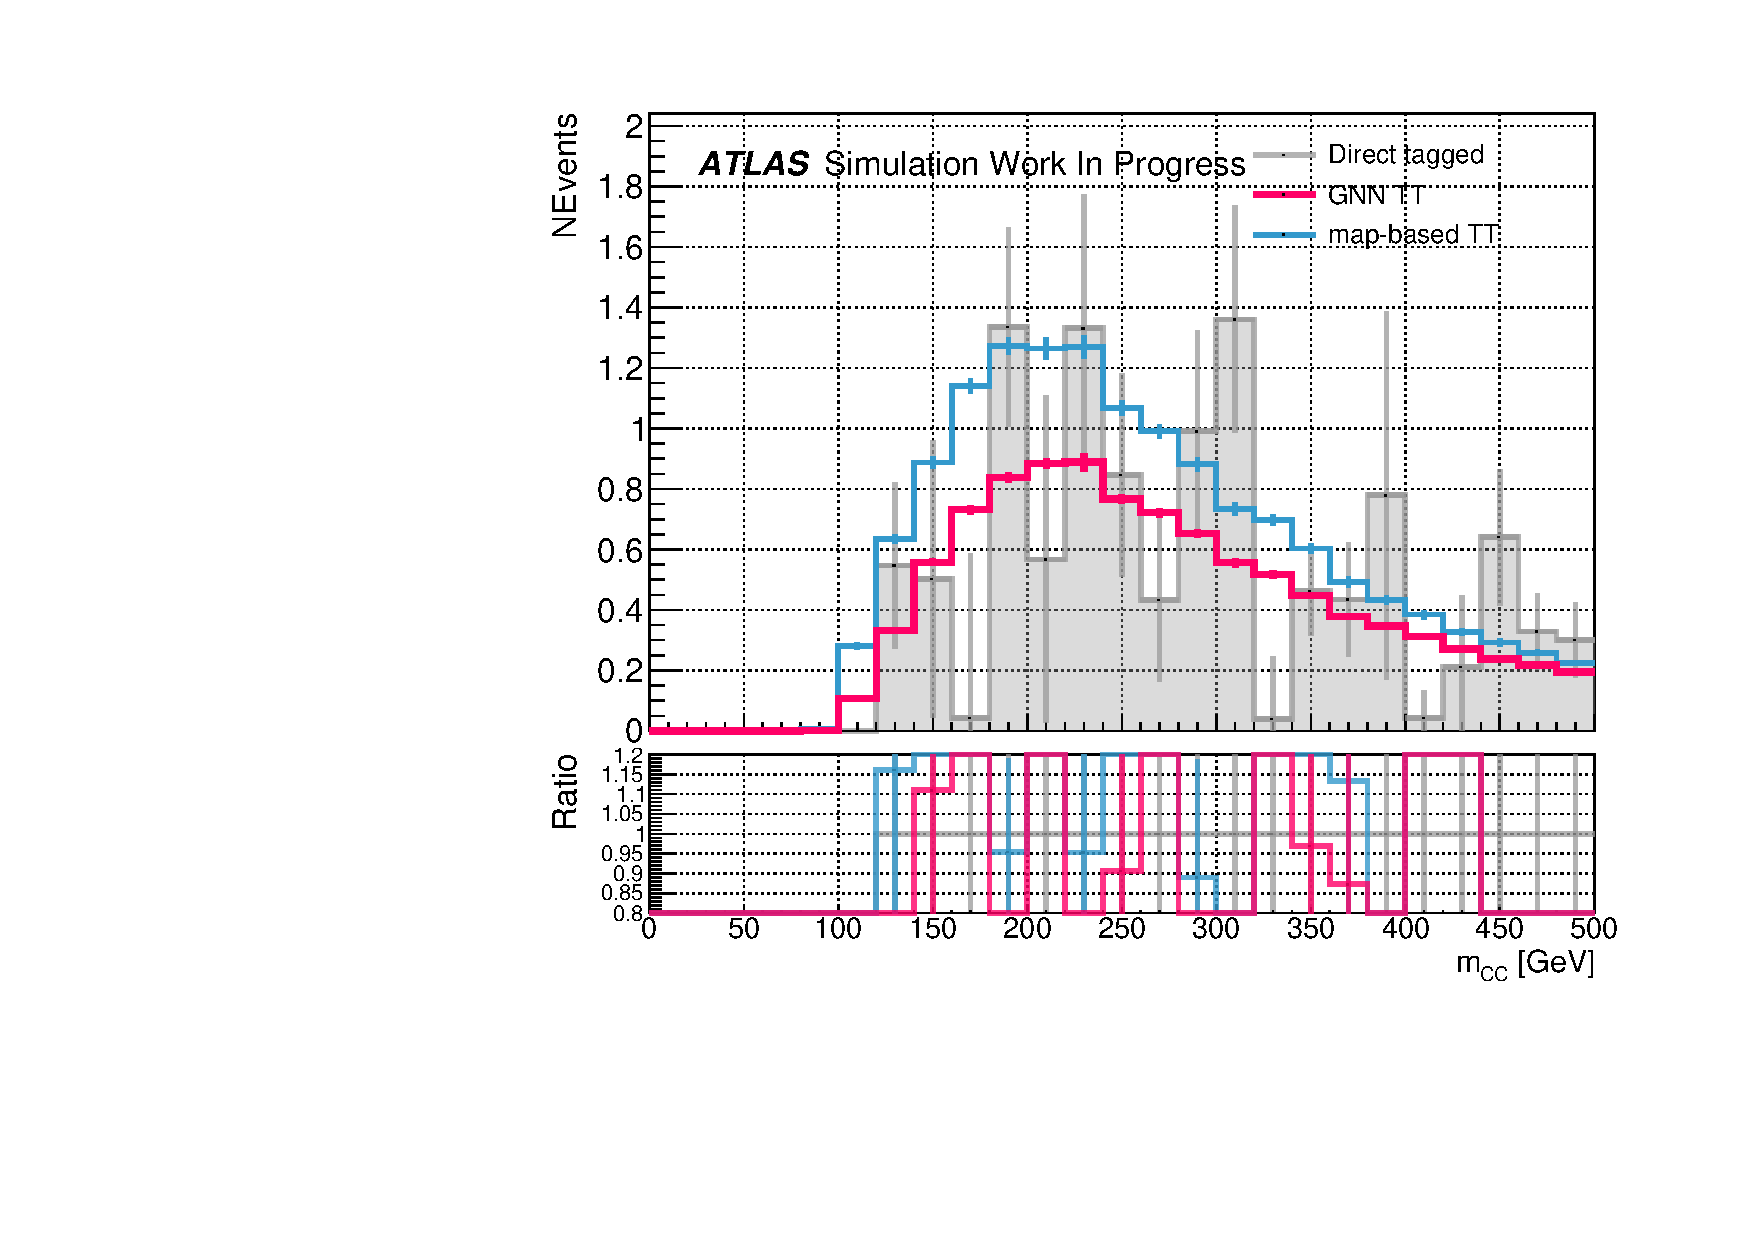
\includegraphics[width=\textwidth]{Images/VH/Tagging/Wl_2tttag2jet_250_400ptv_CRHigh_mCC.pdf}
    \caption{$W+l$ in CRHigh.}
  \end{subfigure}
  \caption{Comparing the tagged $m_{cc}$ distribution for the \vhc\ of the \textsc{Sherpa} 2.2.11 simulated $W+$jets in 1L CRHigh 2-jet region, in the 250 GeV $<$ \ptv\ $< 400$ GeV region. TT stands for truth tagging.}
  \label{fig:truthtaggingW1LVHcc}
\end{figure} 

\section{Tagged-jets corrections}\label{sec-vh-jetcor}
Several corrections to the energy are applied to tagged jet from the previously introduced selection. The objective is to improve the energy resolution of the pair of jets selected to form the Higgs candidate. All jets benefit from a default jet energy calibration called the \textit{Global Sequential Calibration (GSC)} \cite{PhysRevD.96.072002}, as introduced in Section \ref{}. This correction applies to all jets and is not optimal for $b$- and $c$-jets that benefit from special features, motivating the use of additional dedicated corrections for tagged jets. Table \ref{tab:bjetcorrectionregions} summarised the additional corrections presented in this section. % TODO Add a ref to exp chapter, jet section

\begin{table}[!htbp]
    \begin{center}
        \begin{tabular}{c|c|cccc} \hline \hline
          Scheme & lepton channel & muon-in-jet & PtReco & kinematic fit & FSR recovery     \\
          \hline
           \multirow{3}{*}{Resolved \vhb} & 0L & \checkmark & \checkmark &    & \\
                                          & 1L & \checkmark & \checkmark &    & \\  
                                          & 2L & \checkmark & \checkmark (nJet $\geq$ 4) & \checkmark (nJet $\leq$ 3) & \checkmark (nJet $\leq$ 4) \\  
          \hline
           \multirow{3}{*}{\vhc} & 0L & \checkmark &  &    & \\
                                          & 1L & \checkmark &  &    & \\  
                                          & 2L & \checkmark &  & \checkmark (nJet $\leq$ 3) & \checkmark (nJet $\leq$ 4) \\  
          \hline
           \multirow{3}{*}{boosted \vhb}  & 0L & \checkmark &  &    & \\
                                          & 1L & \checkmark &  &    & \\  
                                          & 2L & \checkmark &  &  \checkmark  & \\  
  
          \hline \hline
        \end{tabular}
      \caption{$H$-candidate jet energy correction for different reconstruction strategies.} 
      \label{tab:bjetcorrectionregions}
    \end{center}
  \end{table}
  
\paragraph{\textit{Muon-in-jet} correction} is applied to all events to correct the energy of semi-leptonically decaying $b$- and $c$-jets with a $\mu$. The energy of the $\mu$ is not measured in the calorimeter. For the resolved regime, the closest muon's 4-momentum is added to the jet if their angular separation satisfies \[\Delta R(\textrm{jet}, \mu) < \min\left(0.4, \,0.04 + \frac{10 \textrm{ GeV}}{p_T^{\mu}}\right).\] In the boosted scheme, the angular separation is measured with respect to the track-jet but the muon 4-momentum is added to the large-$R$ jet in case of match.

\paragraph{\textit{PtReco} correction} is applying to account for missing energy from neutrinos in the semi-leptonic decays and for the out-of-cone effect for $b$-jets. It is only applied to $b$-tagged jets in the resolved \vhb\ 0L and 1L channels, and the 4p-jets 2L channel. The correction is derived from the signal samples of \vhb\ by comparing the truth jet $p_T$ and the reconstructed $p_T$ after the muon-in-jet correction. The correction was not found to have a significant effect in the \vhc\ due to the lower likelihood of semi-leptonic decays of $c$-jets.

\paragraph{\textit{Kinematic} fit correction} is applied in the 2L channels of the resolved regime, for the 2- and 3-jet events only. The $ZH \rightarrow\ell\ell b\bar{b} /\ell\ell c\bar{c}$ is fully reconstructed and a kinematif fit is applied to improve the $m_{jj}$ resolution after the muon-in-jet correction. The fit is performed using a likelihood function with terms covering the object resolution, the jet transfer function, a $Z$-mass constraint term and system $p_T$ balance. The boosted 2L channel has a kinematic fit based on a Gaussian term instead. % TODO not clear for boosted. % NOTE not passed to the ETmiss.

\paragraph{\textit{FSR} recovery} is deployed for events with 3 or 4 jets in the resolved regime to improve the resolution of the $m_{bb}$ or $m_{cc}$ peak. Such events are likely to have jets emanating from \glsfirst{fsr}. A continuous cut on the sum $\Delta R_{j, j_1} + \Delta R_{j, j_2}$ of angular separations between a third or fourth jet ($j$) to the Higgs-candidate jet ($j_1$ and $j_2$)  is computed as a function of \ptv. Any jet below the cut is considered a radiation and is added to the closest candidate jet. This effectively corrects the reconstructed mass of Higgs bosons as well as the jet multiplicity, leading to an expected 7\% improvement in \vhb\ \gls{stxs} sensitivity. Due to the possible migration of the \ttb\ background to the sensitive region, this correction is not applied to 0L nor 1L. 

\begin{figure}[h!]
  %\hspace{-4.0cm}
  \centering
  \begin{subfigure}[b]{0.49\textwidth}
    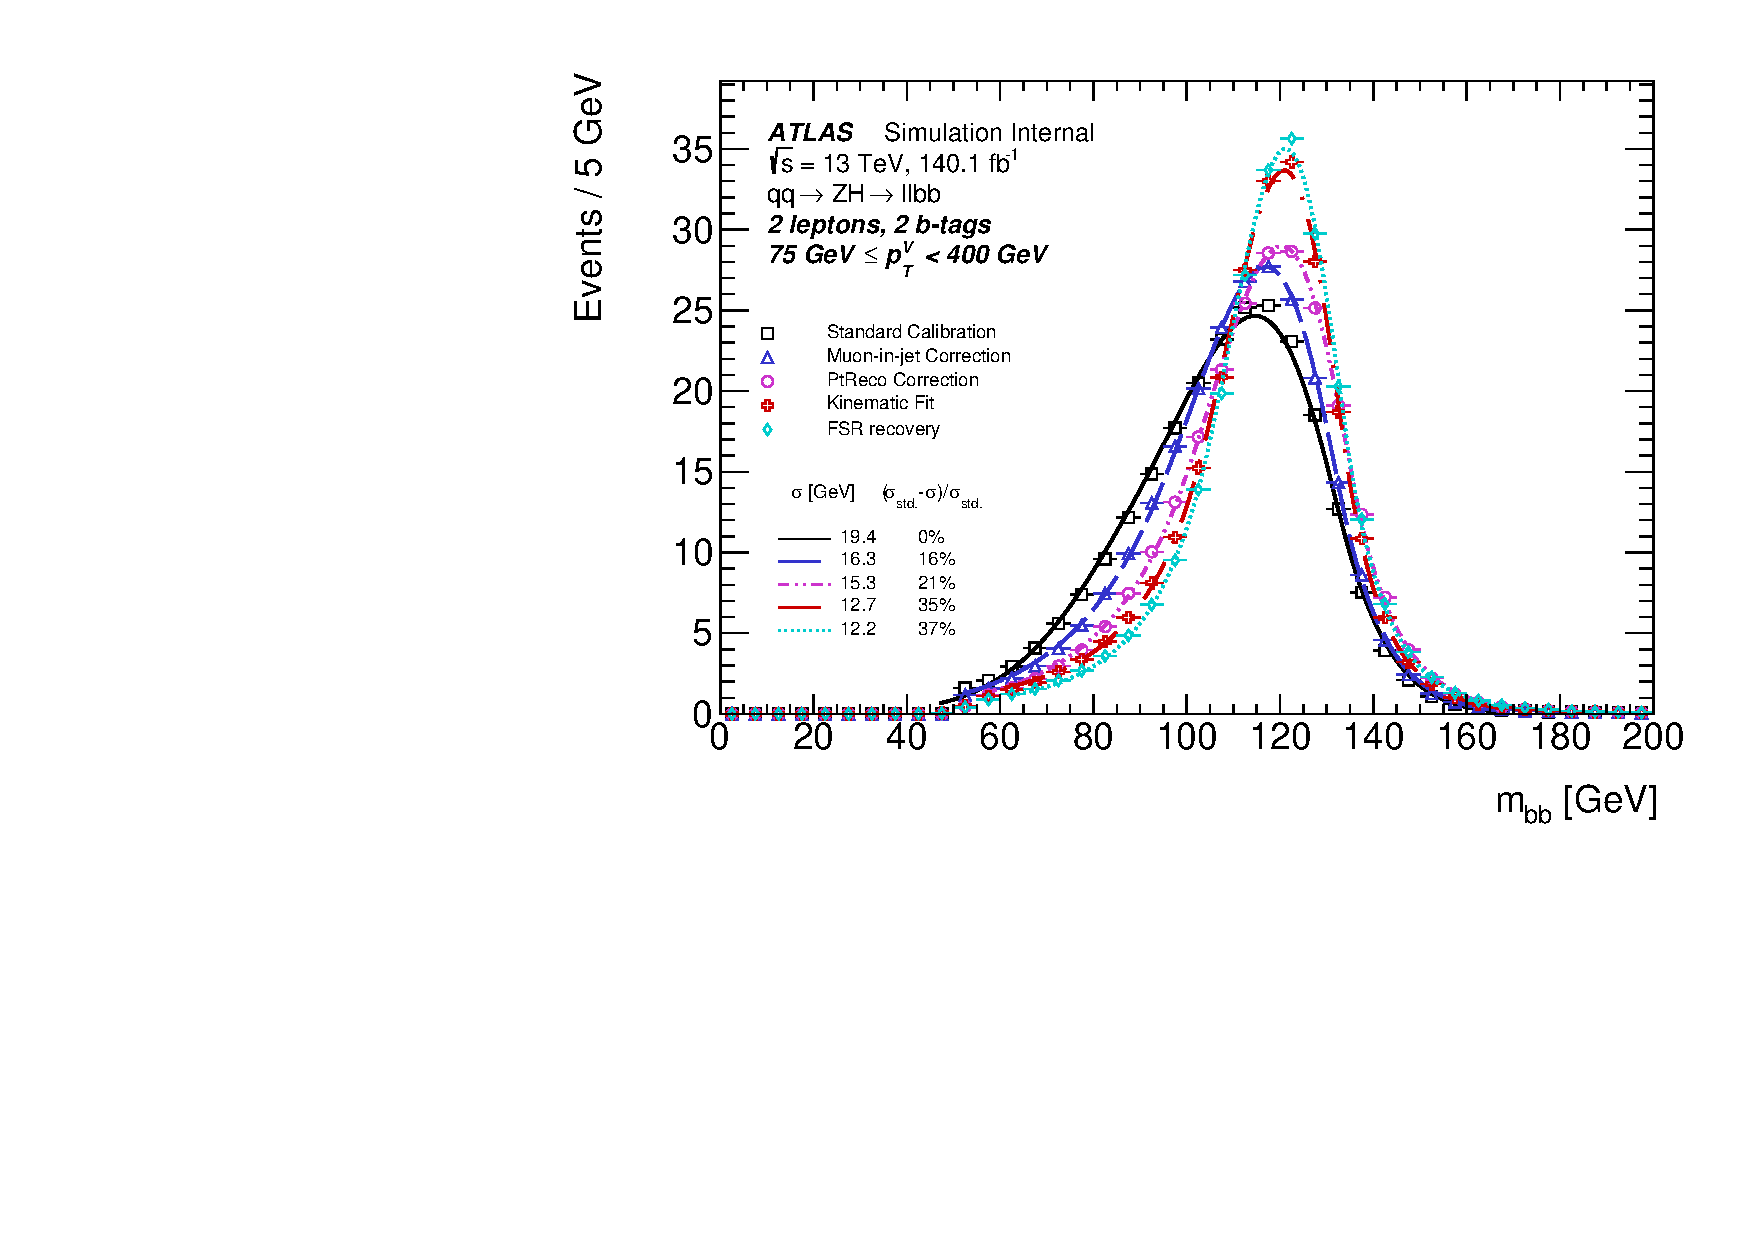
\includegraphics[width=0.98\textwidth]{Images/VH/Correct/CorrectedDist/c_niceMbb_qqZllH125_2tag2pjets_75_400ptv.pdf}
  \caption{Resolved \vhb.} 
  \end{subfigure}
  \begin{subfigure}[b]{0.49\textwidth}
    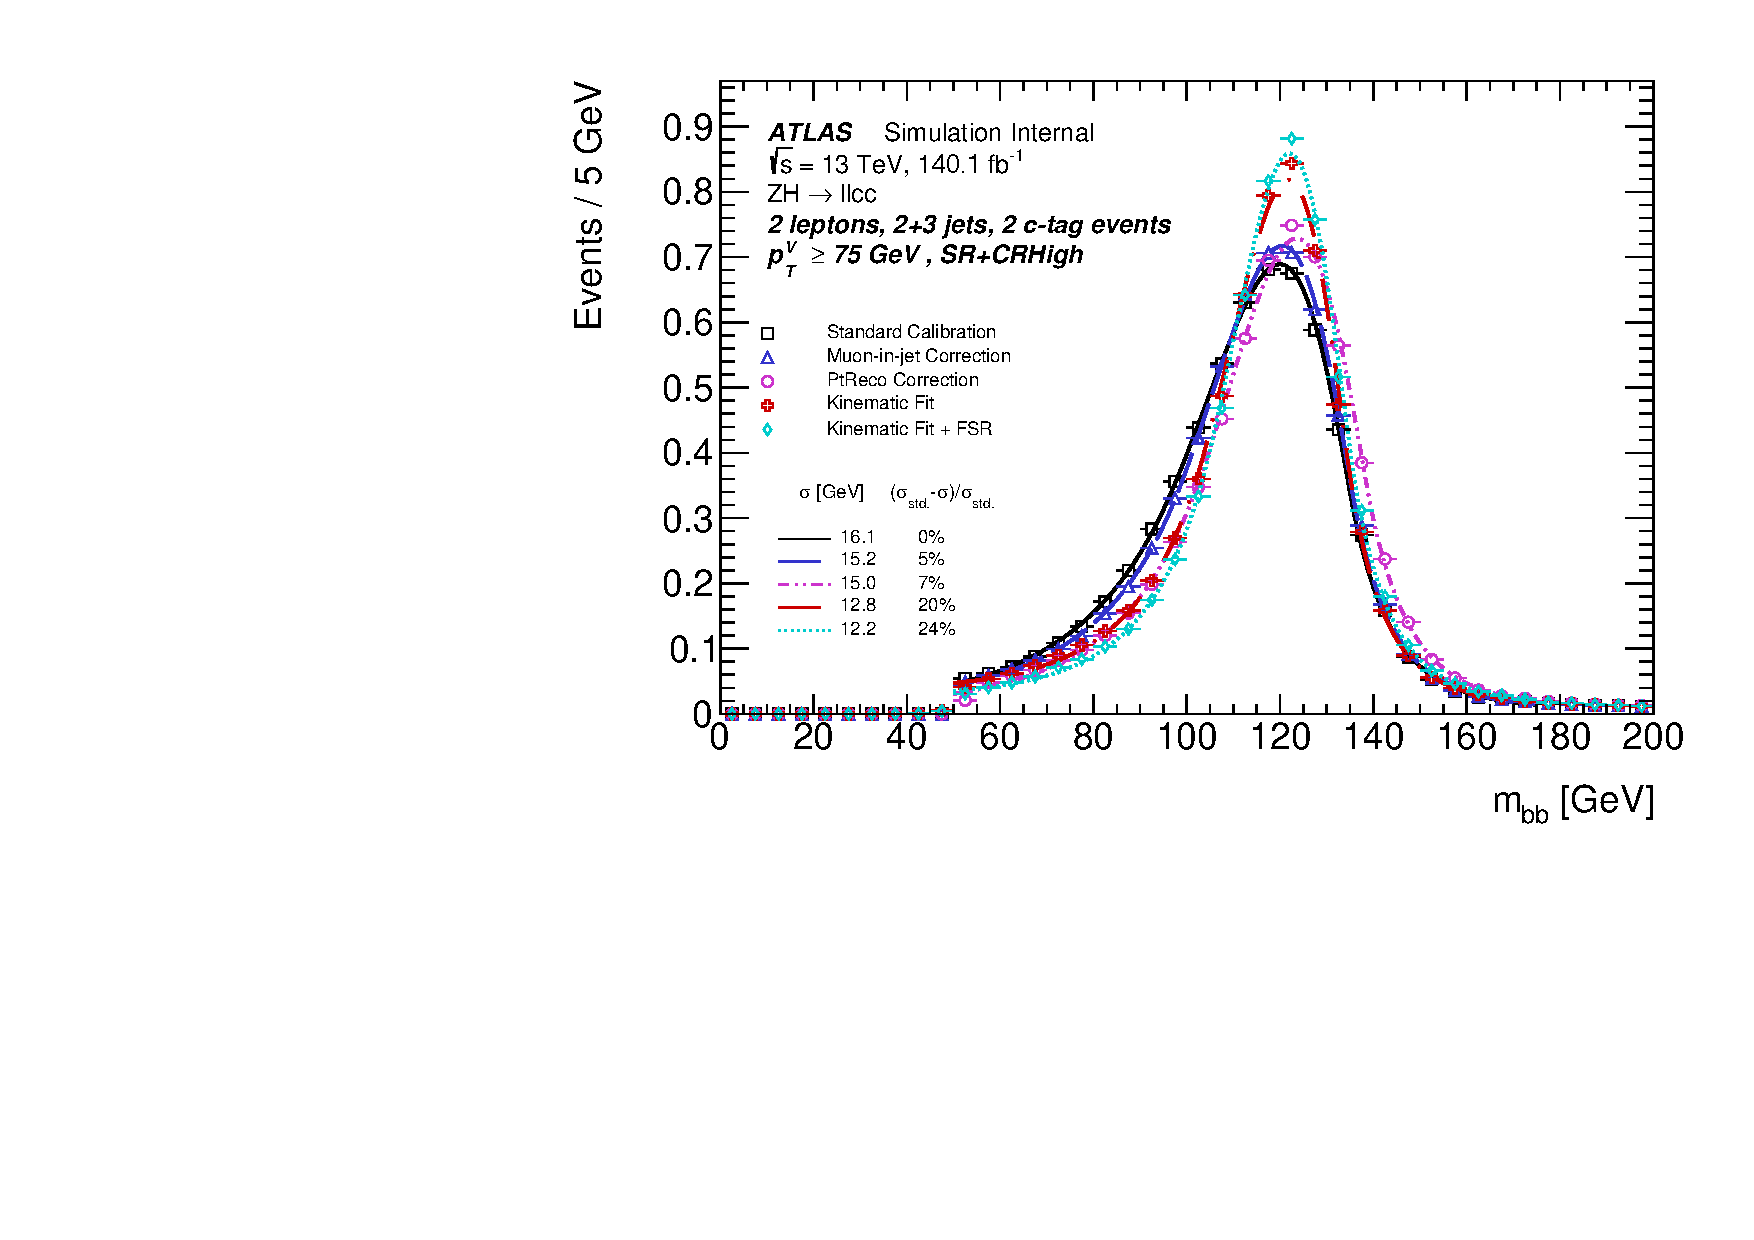
\includegraphics[width=0.98\textwidth]{Images/VH/Correct/CorrectedDist/c_niceMbb_qqZllHcc125_2ctag_75ptv_23j_modified.pdf}
    \caption{Resolved \vhc\ with 2 $c$-tags.}
  \end{subfigure}
  \begin{subfigure}[b]{0.49\textwidth}
    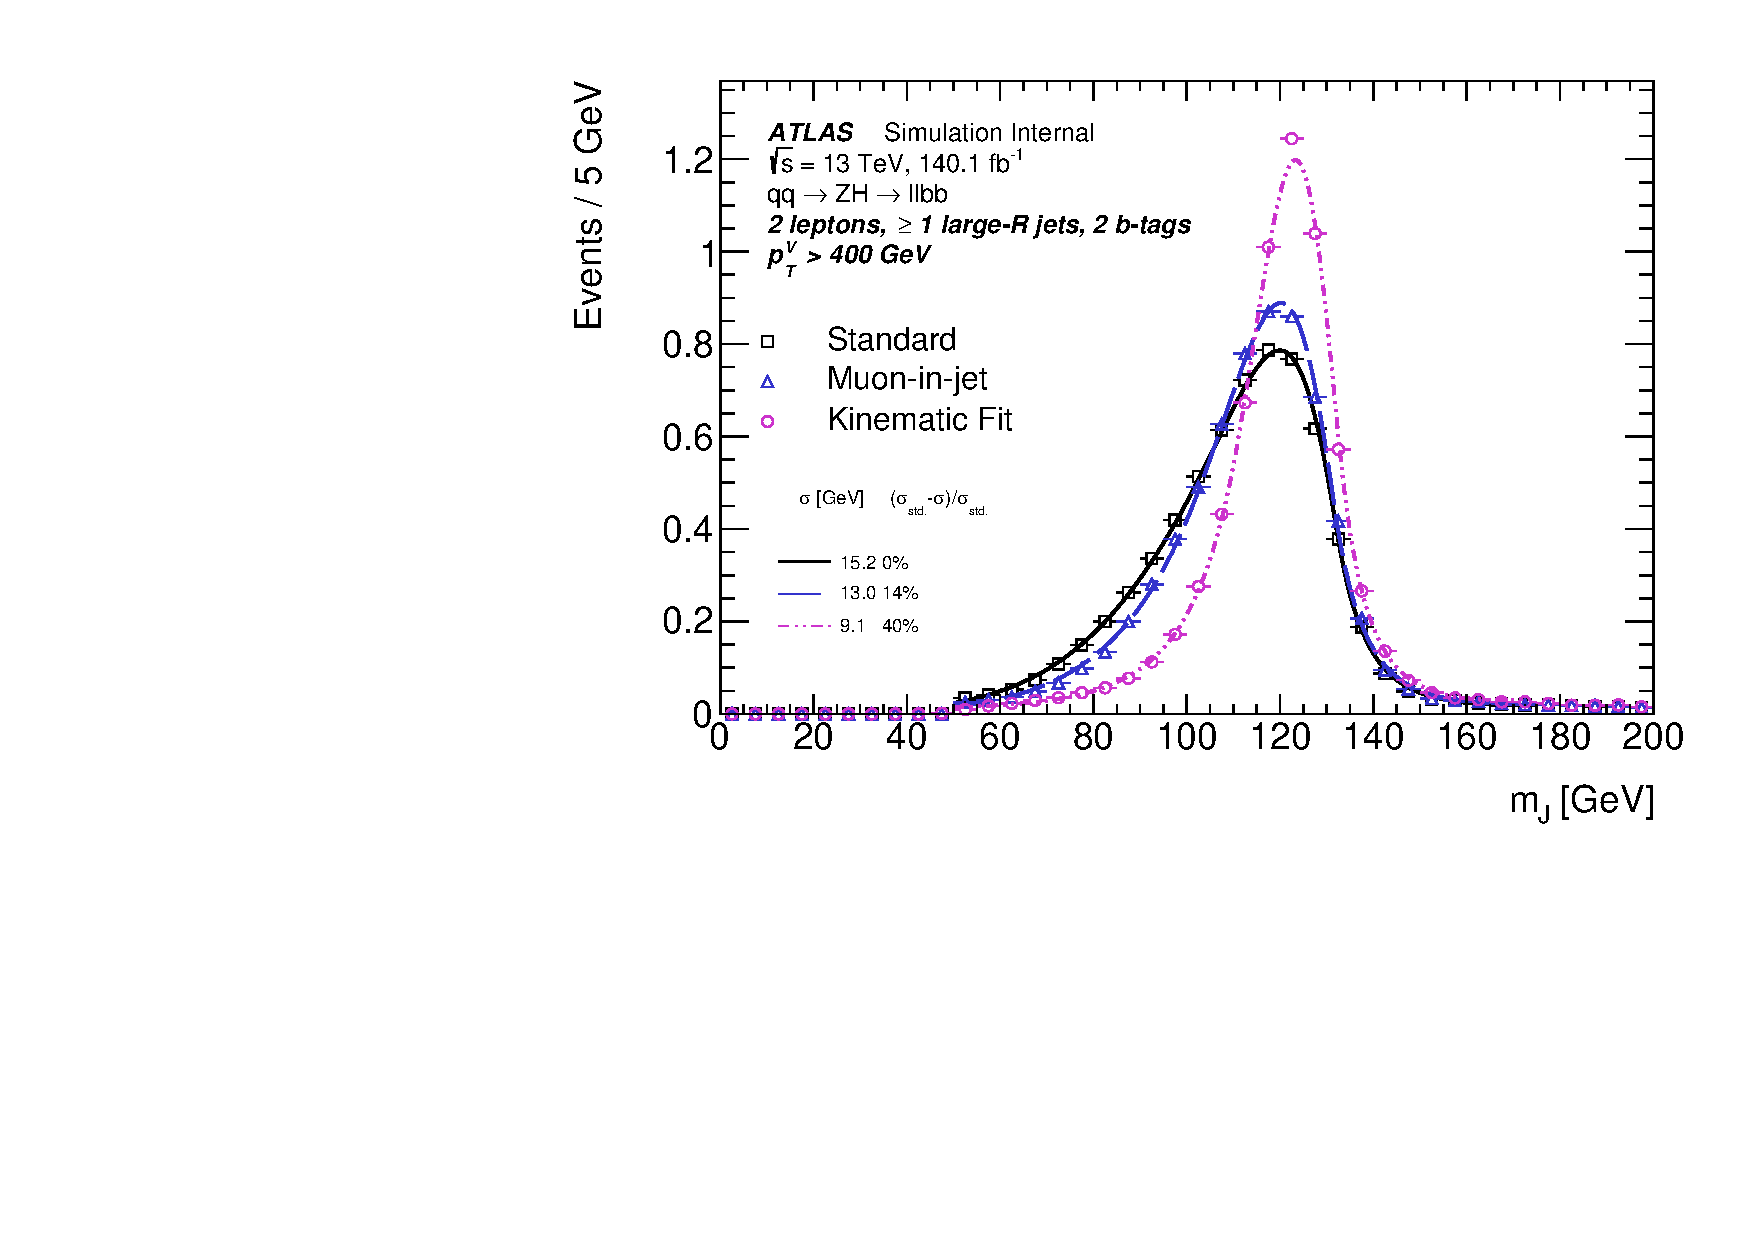
\includegraphics[width=0.98\textwidth]{Images/VH/Correct/CorrectedDist/c_niceMbb_qqZllH125_2tag1pfat_400ptv.pdf}
    \caption{Boosted \vhb.}
  \end{subfigure}
  \caption{Performance of the energy corrections on simulated samples of different analysis schemes in the 2-lepton channels, inclusive in \ptv\ and number of jets.}
  \label{fig:CorrResults}
\end{figure} 

The effect of the different reconstruction techniques is illustrated in Figure \ref{fig:CorrResults} for some selected 2-lepton resolved and boosted \vhb\ and \vhc\ distributions.
